\documentclass[11pt]{article} % do not change this line

\input{BigDataStyle.txt}      % do not change this line

\usepackage{amsmath,amsfonts,amssymb,amsthm,latexsym,graphicx}
\usepackage{booktabs}
\usepackage{listings}
\usepackage{xcolor}
\usepackage{tcolorbox}
\usepackage{algorithm}
\usepackage{algpseudocode}
\usepackage{url}

\emergencystretch=5mm
\tolerance=400
\allowdisplaybreaks[4]

\theoremstyle{plain}

\newtheorem{theorem}{Theorem}[section]
\newtheorem{proposition}[theorem]{Proposition}
\newtheorem{corollary}[theorem]{Corollary}
\newtheorem{lemma}[theorem]{Lemma}
\newtheorem{problem}[theorem]{Problem}

\theoremstyle{definition}

\newtheorem*{remark}{Remark}

\title{Training Small Language Models for Autoformalization to Prolog}

\author{Anonymous}
			
\newcommand{\Programme}{MSc Computer Science (Artificial Intelligence)}

\begin{document}

\maketitle

\declaration

\begin{abstract}

Large language models can produce convincing responses to reasoning tasks while
still making logical errors. Autoformalization offers an alternative approach in which
natural-language statements are translated into a formal representation that can be
checked and executed by a symbolic reasoning system. This project investigates
whether a small language model can be fine-tuned to translate natural-language
reasoning statements into executable Prolog.

A controlled dataset of 2,000 natural-language and Prolog pairs was constructed
across four levels of increasing complexity, covering facts, simple rules,
multi-condition rules and executable reasoning problems. All target programs were
automatically validated using SWI-Prolog. Qwen2.5-1.5B-Instruct was evaluated as a
baseline and subsequently fine-tuned using QLoRA. Performance was measured using
exact-match accuracy, syntactic validity, executability and reasoning correctness.

The baseline model achieved only 0.50\% exact-match accuracy, with 39.70\% of
outputs being syntactically valid and executable. Following fine-tuning, exact-match
accuracy increased to 81.41\%, while syntactic validity and executability both reached
100\%. Error analysis identified recurring weaknesses in complex relational and
multi-condition structures. A targeted refinement dataset of 250 additional examples
was subsequently constructed, after which exact-match accuracy increased to 87.94\%,
with 100\% syntactic validity, executability and reasoning correctness on the 41
reasoning examples. However, because refinement was informed by errors observed
on the test set, the final result is not a fully independent estimate of generalisation.

The results demonstrate that parameter-efficient fine-tuning can enable a small
language model to learn reliable natural-language-to-Prolog translation within a
controlled domain. They also show the value of symbolic execution for distinguishing
syntactic correctness, executability and functional reasoning behaviour from exact
textual agreement.


\end{abstract}


% ============================================================
\clearpage
\section{Introduction}
% ============================================================

Large language models (LLMs) can generate fluent natural language and perform
tasks that appear to require reasoning. However, they can still produce
incorrect or inconsistent answers, particularly when a task requires precise
logical reasoning. A response may appear convincing while containing an invalid
inference or reaching a conclusion that does not follow from the information
provided. This limits the reliability of language models in tasks where
correctness is more important than plausibility.

One approach to improving the reliability of language-model reasoning is
autoformalization. Rather than asking a model to solve a reasoning problem
entirely in natural language, autoformalization translates the problem into a
formal representation that can be checked or executed by another system. This
separates the interpretation of the natural-language problem from the execution
of the resulting symbolic reasoning. If the generated representation can be
executed by a symbolic reasoning system, its properties can be tested directly
rather than assessed solely through the language model's response.

This project investigates autoformalization using Prolog, a logic programming
language based on facts, rules and queries \cite{wielemaker2012swiprolog}.
Prolog provides a useful target representation because generated programs can
be executed using an existing interpreter. A simple example of this translation
is shown below.

\begin{tcolorbox}
\textbf{Natural language:} Every doctor is a professional.

\medskip

\textbf{Prolog:} \texttt{professional(X) :- doctor(X).}
\end{tcolorbox}

More complex statements can similarly be represented using multiple conditions,
relations, inequality and negation. Once a natural-language reasoning problem
has been converted into Prolog, queries can be executed against the generated
program to determine whether the expected conclusions follow.

The project focuses specifically on small language models (SLMs) rather than
substantially larger models. Smaller models require fewer computational
resources and can be fine-tuned on consumer hardware, but their lower capacity
raises the question of whether they can reliably learn the precise
correspondence between natural-language statements and symbolic programs. This
leads to the central research question: to what extent can a small language
model be fine-tuned to translate natural-language reasoning problems into
syntactically valid, executable and logically correct Prolog programs?

To investigate this question, a controlled dataset of natural-language and
Prolog pairs was constructed. The dataset contains 2,000 examples divided
across four levels of increasing complexity. These range from individual facts
and simple rules to rules containing multiple conditions and examples requiring
a Prolog query to be evaluated. The dataset was automatically validated using
SWI-Prolog to ensure that the target programs were syntactically valid and
executable. Reasoning examples were additionally checked to ensure that their
queries produced the expected results. A group-aware training, validation and
test split was used to reduce leakage between closely related examples.

The experiments use Qwen2.5-1.5B-Instruct as the small language model \cite{qwen25}. The
unmodified model was first evaluated on the held-out test set to establish a
baseline. Its performance demonstrated the difficulty of the task without
task-specific training: only 0.5\% of generated programs exactly matched the
expected Prolog, while 39.7\% were syntactically valid and executable. The model
was subsequently fine-tuned on the constructed dataset using QLoRA. Following
fine-tuning, exact-match accuracy increased to 81.41\%, while all generated
programs were syntactically valid and executable.

The remaining failures were examined through error analysis rather than
treating aggregate accuracy as the only measure of performance. This analysis
identified several recurring weaknesses, particularly in more complex
multi-condition rules and specific relational structures. These observations
were used to construct a targeted refinement dataset containing 250 additional
examples focused on areas in which the first fine-tuned model performed poorly.

A second version of the model was then trained using this additional data and
evaluated on the same test set. The final model achieved an exact-match accuracy
of 87.94\%, with 100\% syntactic validity, 100\% executability and correct results on
all 41 reasoning examples in the test set. As the refinement data were informed by
error patterns observed on this test set, these final results are treated as refinement
results rather than as a fully independent estimate of generalisation.


These results also demonstrate why several evaluation criteria are useful for
autoformalization. Exact string matching provides a strict measure of whether a
generated program is identical to the reference representation, but it does not
by itself indicate whether the generated output is usable. Syntax validation
determines whether the output forms valid Prolog, while execution determines
whether it can be successfully processed by the Prolog interpreter. Reasoning
evaluation provides an additional functional measure by testing whether
generated programs produce the expected answer to a query. This distinction is
important because a generated symbolic representation can differ from a
reference string while still retaining useful executable behaviour.

The main contribution of this project is an end-to-end investigation of
small-model autoformalization to Prolog. It includes the construction and
validation of an NL to Prolog dataset, the establishment of an untuned baseline,
parameter-efficient fine-tuning of a 1.5-billion-parameter language model,
execution-based evaluation using SWI-Prolog, systematic analysis of translation
errors and targeted refinement based on the observed failures. The experiments
show that task-specific fine-tuning can substantially improve a small language
model's ability to generate valid executable Prolog, while also identifying
translation structures for which exact generation remains more difficult.

The remainder of this dissertation develops this investigation in detail:

\begin{itemize}
    \item Chapter 2 introduces the relevant background and related work in
    language-model reasoning, autoformalization, Prolog and
    parameter-efficient fine-tuning.

    \item Chapter 3 describes the construction, validation and splitting of
    the NL to Prolog dataset.

    \item Chapter 4 presents the model, training procedure, system design and
    evaluation methodology.

    \item Chapter 5 reports the baseline, fine-tuning, error analysis and
    refinement experiments.

    \item Chapter 6 discusses the significance and limitations of the results,
    including the distinction between exact-match and execution-based
    evaluation.

    \item Chapter 7 summarises the findings of the project and identifies
    directions for future work.
\end{itemize}


% ============================================================
\clearpage
\section{Background and Related Work}
% ============================================================

This chapter introduces the concepts and previous research most relevant to the
project. The project lies at the intersection of language models, symbolic
reasoning and autoformalization. This central approach uses a language model to
translate natural-language statements into Prolog rather than requiring the
model to perform the entire reasoning process directly in natural language.
This section therefore considers language-model reasoning, neuro-symbolic
approaches, Prolog as a target formal language, existing reasoning datasets,
and parameter-efficient methods for adapting smaller language models.


\subsection{Language Models and Logical Reasoning}

Transformer-based language models learn statistical relationships between
tokens from large collections of text. This enables modern models to perform a
wide range of tasks through natural-language prompting, including question
answering, code generation and tasks that appear to require multi-step
reasoning. However, generating a plausible sequence of tokens is not equivalent
to following a formally defined reasoning procedure. This distinction becomes
important when the correctness of each inference matters.

Research into logical reasoning with language models predates many current
large language models. Clark et al.~\cite{clark2020ruletaker} introduced RuleTaker, in which
transformer models were trained to answer questions from natural-language facts
and rules. This demonstrated that transformer models could achieve high
accuracy on synthetically generated logical reasoning problems and could
generalise to some problems requiring deeper inference chains than those
encountered during training. The authors described these models as ``soft
theorem provers'', since the reasoning process was learned from examples rather
than performed through an explicit symbolic inference system.

The RuleTaker results show that transformer models can learn patterns
corresponding to deductive reasoning. However, learning the behaviour of
a reasoning process is not equivalent to executing a formal reasoning
procedure. A neural model may produce the correct answer without
providing a representation that can independently be checked by a
deterministic solver. This motivates approaches in which language
understanding and formal inference are separated.

A related line of research has therefore investigated neuro-symbolic reasoning,
combining the flexibility of neural language models with the explicit inference
procedures of symbolic systems. This approach does not require the language
model to both interpret a problem and solve it; instead, the language model can
act as a translator or semantic parser. The resulting formal representation is
then passed to a symbolic system responsible for inference.


\subsection{Autoformalization}

Autoformalization is the automatic translation of informal natural-language
statements into a formal representation. This was investigated directly by
Wu et al.~\cite{wu2022autoformalization}, who used large language models to
translate mathematical statements into Isabelle/HOL. Their experiments showed that language models
could correctly formalize a portion of mathematical competition problems and
that the generated formalizations could subsequently support automated theorem
proving. These results showed that language models could serve as an interface
between informal human language and representations suitable for formal verification.

The importance of autoformalization is that formal output can be subjected to
checks that are unavailable for ordinary natural-language responses. This means
that a natural-language answer may be grammatically correct and persuasive
while still containing an invalid inference. A formal representation instead
has a defined syntax and semantics and can be processed by an appropriate
interpreter, theorem prover or solver. This translation may still be incorrect,
but errors can potentially be detected through parsing, execution or comparison
with expected behaviour.

Pan et al.~\cite{pan2023logiclm} developed this idea further with Logic-LM, a
framework in which an LLM first translates a natural-language reasoning problem
into a symbolic formulation. A deterministic symbolic solver then performs the actual
inference. Logic-LM was evaluated on five reasoning datasets, including
ProofWriter~\cite{tafjord2021proofwriter} and FOLIO, and produced substantial
improvements over both standard prompting and chain-of-thought prompting. This
framework also included a refinement stage that used error messages from the
symbolic solver to revise incorrect formalizations.

A similar approach is used by Olausson et al.~\cite{olausson2023linc} in LINC,
or Logical Inference via Neurosymbolic Computation. This system treats the language model
as a semantic parser that translates natural-language premises and conclusions
into first-order logic. Deductive reasoning is then delegated to an external
theorem prover. Their experiments on ProofWriter~\cite{tafjord2021proofwriter}
and FOLIO found that this separation could outperform direct chain-of-thought
reasoning. LINC also produced strong results when using an open-source model
smaller than the largest proprietary models evaluated in the study.

These systems support the central principle behind the present project: a
language model does not necessarily need to perform every part of logical
reasoning internally. This allows it to perform the task for which
natural-language models are particularly useful, interpreting language, while
a symbolic system handles formally defined inference.


\subsection{Prolog as a Symbolic Representation}

This project uses Prolog as the target language for autoformalization. Prolog is
a logic programming language in which programs are primarily expressed using
facts and rules. This knowledge base can then be queried to determine whether
particular conclusions follow from those facts and rules.

For example, the statements:

\begin{tcolorbox}
\begin{lstlisting}[language=Prolog]
doctor(mary).
professional(X) :- doctor(X).
\end{lstlisting}
\end{tcolorbox}

represent the fact that Mary is a doctor and the rule that every doctor is a
professional. A query such as:

\begin{tcolorbox}
\begin{lstlisting}[language=Prolog]
professional(mary).
\end{lstlisting}
\end{tcolorbox}

can then be evaluated by the Prolog system. Prolog uses mechanisms including
unification and proof search to determine whether a query follows from the
available knowledge base.

This makes Prolog useful for the current project in two ways. First, its
relatively compact syntax provides a structured target for natural-language
translation. This allows natural-language statements describing properties and
relations to be represented as predicates, while conditional statements can be
represented as rules. Second, generated programs can be executed. This makes
it possible to distinguish several forms of correctness: whether the generated
text exactly matches a reference program, whether it is syntactically valid
Prolog, whether it executes successfully, and whether executing a query
produces the expected result.

Recent neuro-symbolic work has also explored Prolog specifically. Yang et
al.~\cite{yang2025neurosymbolic} use Prolog interpreters as part of a
neuro-symbolic reasoning framework and argue that, once a problem has been
correctly translated into Prolog, the interpreter can provide reliable symbolic
reasoning and expose its intermediate search process. More recently, Mellgren
et al.~\cite{mellgren2026prolog} investigated training Qwen2.5-3B-Instruct to
use Prolog as an external reasoning tool. This work
considered execution, syntax and semantic correctness as training signals and
highlighted a distinction between obtaining a correct final answer and
producing a genuinely auditable symbolic program.

This distinction is relevant to the evaluation performed in this project. A
model that produces valid Prolog has achieved something different from a model
that merely produces the expected final answer. This executable symbolic
representation creates an intermediate artefact that can itself be inspected
and evaluated.


\subsection{Natural-Language Reasoning Datasets}

Training a model to translate natural language into a formal representation
requires paired examples containing linguistic statements and their
corresponding logical structures. This means that existing logical reasoning
datasets provide useful examples of how controlled reasoning problems can be
constructed.

RuleTaker uses synthetic natural-language theories containing facts and rules,
with questions requiring models to determine whether conclusions follow from
them. This allows reasoning depth and logical structure to be controlled
systematically. Bao et al.~\cite{bao2022pararule} extended this direction through
PARARULE-Plus, a large dataset designed for multi-step deductive reasoning over
natural language. This dataset contains reasoning chains at depths from two to
five and approximately 400,000 examples across its different depth levels. It
uses entities such as people and animals together with relationships and
attributes and follows a closed-world reasoning setting.

These datasets influenced the design space of the current project,
particularly the use of controlled natural-language templates and progressively
more complex reasoning structures. However, this objective differs from
ordinary question answering over these datasets. The desired model output is
not simply a true or false label. Instead, the model must generate the
underlying Prolog representation itself.

For this reason, a dedicated NL to Prolog dataset was constructed rather than
directly training on PARARULE-Plus. This provides precise control over the
expected Prolog syntax, predicate structures and difficulty levels and allows
every target program to be automatically checked with the same Prolog
implementation used during evaluation. This dataset construction is described
in Chapter 3.


\subsection{Small Language Models and Parameter-Efficient Fine-Tuning}

Many autoformalization and neuro-symbolic studies use comparatively large
language models. This project instead investigates whether a much smaller model
can acquire the required translation behaviour through targeted fine-tuning.

The selected model is Qwen2.5-1.5B-Instruct, part of the Qwen2.5 family. Its
technical report describes a family of models offered at several parameter
scales and improved through both pre-training and post-training. The
instruction-tuned variants are designed to follow user instructions and
generate structured responses, making the 1.5-billion-parameter version a
suitable starting point for a constrained generation task.

Fine-tuning all parameters of a language model can require substantial memory
and computational resources. This requirement is reduced by Low-Rank
Adaptation (LoRA), introduced by Hu et al.~\cite{hu2021lora}, which freezes the original
model weights and introduces a smaller number of trainable low-rank matrices.
Only these additional parameters need to be optimised for the downstream task.
This substantially reduces the number of trainable parameters while retaining
much of the benefit of task-specific adaptation.

QLoRA, introduced by Dettmers et al.~\cite{dettmers2023qlora}, extends this
approach by combining LoRA with quantisation. This method stores the pretrained model using 4-bit
quantised weights while gradients are propagated into the trainable LoRA
adapters. Dettmers et al. demonstrated that this approach can greatly reduce
memory requirements while maintaining competitive fine-tuning performance.

This makes QLoRA particularly appropriate to the aims of this project because
it makes fine-tuning feasible on limited hardware. The investigation can
therefore focus on whether a small model can learn NL to Prolog translation
without requiring the computational resources associated with full fine-tuning
or substantially larger language models.


\subsection{Position of This Project}

Previous research provides a lot of foundation for this project. Autoformalization
research establishes that language models can translate informal statements
into formal languages, while Logic-LM and LINC separate language interpretation
from symbolic inference. RuleTaker and PARARULE-Plus provide examples of
controlled datasets for studying logical reasoning, and recent Prolog-based work
explores executable logic programs as an interface between language models
and formal reasoning.

Despite these similarities, the present project differs from this previous work
in its primary experimental focus. RuleTaker and PARARULE-Plus primarily
evaluate reasoning over natural-language facts and rules rather than
generation of an executable formal representation. Logic-LM and LINC use
language models as components within neuro-symbolic reasoning pipelines,
whereas this project isolates the formalization stage as the principal learning
task. The Prolog-based work of Mellgren et al. similarly demonstrates the value
of executable symbolic programs, but uses a larger Qwen2.5-3B-Instruct model
and investigates Prolog as an external reasoning tool. In contrast, the present
project examines direct task-specific adaptation of Qwen2.5-1.5B-Instruct for
NL to Prolog translation.

The central question is therefore not whether a large general-purpose language
model can be prompted to produce symbolic representations, but whether a
1.5-billion-parameter model can be explicitly trained to perform NL to Prolog
translation reliably within a controlled domain. The generated output is evaluated
at several levels, separating exact textual agreement from syntactic validity,
executability and reasoning correctness. This allows the experiments to distinguish
between learning the surface form of Prolog, producing executable programs
and preserving sufficient logical structure to support correct symbolic inference.

% ============================================================
\clearpage
\section{Dataset Design and Construction}
% ============================================================

The dataset is a central component of this project because fine-tuning requires
paired examples showing the relationship between natural-language statements and
their expected Prolog representations. Existing datasets such as RuleTaker,
ProofWriter \cite{tafjord2021proofwriter} and PARARULE-Plus provide large collections of controlled
natural-language reasoning problems. However, their primary objective is usually
to determine whether a conclusion follows from a collection of facts and rules
rather than to train a model to generate executable Prolog directly. A dedicated
dataset was therefore constructed for this project.

The final dataset contains 2,000 natural-language and Prolog examples divided
into four levels of increasing complexity. The design aimed to provide a
controlled progression from basic translation to more complex rules and
executable reasoning. Each example was generated together with metadata
describing its level, category and template group. The complete dataset was
validated using SWI-Prolog before being divided into training, validation and
test sets.

\subsection{Dataset Design}

Synthetic generation was chosen because it provides direct control over both
sides of each training pair. Similar approaches have previously been used for
logical reasoning datasets. RuleTaker generates theories containing
natural-language facts and rules from a configurable grammar and derives labels
using a reasoning engine. ProofWriter \cite{tafjord2021proofwriter} extends this style of dataset with rule
bases, questions and proofs of different depths. PARARULE-Plus similarly
generates large numbers of natural-language reasoning examples involving people,
animals, attributes and relationships.

Together, these approaches demonstrate the usefulness of controlled synthetic
data when the underlying logical structure of every example must be known. The
same principle was used in this project, although the target differs. Rather
than generating a natural-language theory followed by a classification label,
each example pairs natural language directly with its expected Prolog program.

An example of a simple pair is:

\begin{tcolorbox}

\textbf{Natural language:} Mary is a doctor.

\medskip

\textbf{Prolog:} \texttt{doctor(mary).}

\end{tcolorbox}

A rule can be represented as:

\begin{tcolorbox}

\textbf{Natural language:} Every doctor is a professional.

\medskip

\textbf{Prolog:} \texttt{professional(X) :- doctor(X).}

\end{tcolorbox}

The direct pairing makes the required model behaviour explicit. The model
receives a natural-language statement and is trained to return only its Prolog
representation.

The dataset was generated programmatically rather than written manually.
Templates defined corresponding natural-language and Prolog structures, while
entities and predicates were varied to produce individual examples. This reduced
the amount of manual annotation required and ensured that the intended symbolic
representation was known at generation time.

The overall generation procedure is summarised in
Algorithm~\ref{alg:dataset_generation}. Examples were generated according
to the requirements of each difficulty level, with predefined templates
controlling the relationship between the natural-language statement and its
corresponding Prolog representation. Reasoning examples additionally
included a query and an expected result.

\begin{algorithm}[ht]
\caption{NL to Prolog Dataset Generation}
\label{alg:dataset_generation}
\begin{algorithmic}[1]
\Require Level specifications, NL templates, Prolog templates,
         entity names and predicates
\Ensure Dataset of NL to Prolog examples

\State Initialise empty dataset

\For{each difficulty level}
    \State Load the templates associated with the level

    \While{target number of examples has not been reached}
        \State Select a template
        \State Select the required entities and predicates
        \State Generate the natural-language statement
        \State Generate the corresponding Prolog representation
        \State Assign the level, category and template group

        \If{the example requires reasoning}
            \State Generate the associated query
            \State Assign the expected query result
        \EndIf

        \If{the generated example is unique}
            \State Add the example to the dataset
        \EndIf
    \EndWhile
\EndFor

\State Save the completed dataset
\end{algorithmic}
\end{algorithm}

However, purely template-based generation introduces the risk that a model
learns surface patterns rather than the underlying translation. To reduce this
effect, multiple natural-language forms, entities and predicate combinations
were included. Examples were also assigned to template groups so that closely
related examples could later be kept within the same dataset split.

\subsection{Dataset Structure}

Each dataset entry was stored in JSONL format. The principal fields were
\texttt{id}, \texttt{level}, \texttt{category}, \texttt{natural\_language},
\texttt{prolog}, \texttt{template\_group} and \texttt{nl\_template}. Reasoning
examples additionally contain a \texttt{query} and an
\texttt{expected\_result}.

The \texttt{id} provides a unique identifier that allows individual examples to
be traced during validation and error analysis. The \texttt{level} records the
intended difficulty of the example, while \texttt{category} describes the type
of translation. \texttt{natural\_language} contains the model input and
\texttt{prolog} contains the expected output.

The \texttt{template\_group} field identifies examples derived from the same
underlying logical pattern. This became important during splitting because two
sentences can use different names or surface wording while representing almost
the same translation task. The \texttt{nl\_template} field provides additional
information about the linguistic form from which the example was generated.

Reasoning examples contain two further fields. The \texttt{query} specifies the
Prolog goal that should be executed after loading the generated program, while
\texttt{expected\_result} records whether the query should succeed. These fields
allow the dataset to test functional reasoning behaviour in addition to
translation.

JSONL was used because each example can be processed independently while
retaining structured metadata. It also allowed the same records to be reused
throughout generation, validation, splitting, training and evaluation.

\subsection{Difficulty Levels}

The 2,000 examples were divided into four levels. Each level introduces
additional structural complexity.

\textbf{Level 1} contains 500 facts. These examples establish the simplest
correspondence between natural-language statements and Prolog predicates. Both
unary predicates, such as properties of a single entity, and binary predicates
describing relationships between two entities were included.

\textbf{Level 2} contains 600 simple rules. These examples introduce variables
and implication. A natural-language statement such as ``Every doctor is a
professional'' must be converted into a Prolog rule with the conclusion before
\texttt{:-} and its condition afterwards. This requires more structural
transformation than copying information into a fact.

\textbf{Level 3} contains 500 multi-condition rules. These introduce
conjunctions and more complex logical structures, including inequality and
negation-as-failure. For example, a rule may require several conditions to be
satisfied before its conclusion follows. The level was designed to test whether
the model could preserve multiple relationships and variables while producing
valid Prolog syntax.

\textbf{Level 4} contains 400 reasoning examples. These contain sufficient facts
and rules for a specified query to be executed. The expected result of the query
is stored alongside each example. Evaluation can therefore move beyond checking
whether the generated output resembles the reference representation and test
whether the resulting program supports the expected inference.

The use of progressively more difficult structures follows a similar principle
to datasets such as ProofWriter \cite{tafjord2021proofwriter} and PARARULE-Plus, where reasoning problems are
organised according to inference depth. The levels in this project are not
equivalent to their reasoning depths because they measure translation complexity
rather than only the number of inference steps. Nevertheless, both approaches
provide a controlled way to examine where model performance begins to degrade.

\subsection{Vocabulary and Template Generation}

A controlled vocabulary was used when generating examples. Twenty-six entity
names were included, such as \texttt{ash}, \texttt{mary}, \texttt{olivia},
\texttt{ray}, \texttt{violet} and \texttt{zelda}. Predicates were divided into
unary and binary forms. Unary predicates represented properties or classes,
while binary predicates represented relationships such as \texttt{calls/2},
\texttt{admires/2}, \texttt{parent/2}, \texttt{likes/2},
\texttt{teacher\_of/2} and \texttt{student\_of/2}.

The controlled vocabulary was intended to keep the emphasis on learning the
mapping between linguistic and logical structure. RuleTaker and PARARULE-Plus
use a related strategy, combining limited collections of entities, attributes
and relationships to create large numbers of controlled reasoning problems.

Templates were created for each category and instantiated with different
entities and predicates. More complex templates explicitly controlled variable
placement because reversing the arguments of a binary predicate can change the
meaning of the generated program. This was particularly important for
relationships such as \texttt{parent/2} and \texttt{teacher\_of/2}.

Several issues were discovered during dataset development. These included
incorrect article selection such as ``a'' versus ``an'', an incorrect predicate
mapping, duplicated Level 3 structures, and errors in the expected outcomes of
some reasoning examples. The problems were corrected before the dataset was
frozen. Iterative checking was important because systematic errors in
automatically generated targets would otherwise teach the model incorrect
translations.

\subsection{Automated Prolog Validation}

Automatic validation was included as part of the dataset construction pipeline.
Each generated target was written to a temporary Prolog file and checked using
SWI-Prolog. Examples were tested for both syntactic validity and successful
loading by the interpreter.

Reasoning examples underwent an additional check. After loading the facts and
rules, the associated query was executed and its result was compared with
\texttt{expected\_result}. This ensured that the expected answer stored in the
dataset agreed with the behaviour of the Prolog program.

The use of a symbolic engine to derive or verify dataset labels has precedent in
related work. RuleTaker's generator, for example, can pass generated theories
through a reasoning engine to obtain gold labels. The approach used here applies
the same general principle directly to the target representation: because Prolog
is executable, the generated target programs can be checked before they are used
for model training.

Validation initially revealed errors in the generated data, particularly in the
reasoning examples. The errors were corrected and the validation process was
repeated until all 2,000 examples were syntactically valid and executable, and
all 400 reasoning examples produced their expected results. The validated
dataset was then frozen as the first dataset version so that subsequent
experiments would operate on a consistent collection of examples.

\subsection{Training, Validation and Test Split}

The validated dataset was divided into training, validation and test sets using
an approximately 80/10/10 split. This produced 1,597 training examples, 204
validation examples and 199 test examples. A fixed random seed of
\texttt{4242564} was used so that the split could be reproduced.

A purely random split at the level of individual examples was avoided.
Template-generated datasets can contain examples that differ only in entity
names or minor wording. Placing closely related examples in both training and
test data would make evaluation less informative because the model could
encounter almost the same pattern during training.

Examples were therefore grouped using \texttt{template\_group}, and groups
rather than individual examples were assigned to dataset splits. This reduces
direct leakage between structurally related examples and provides a more
meaningful test of whether the model has learned mappings that extend beyond
individual generated examples.

The test set was kept fixed throughout the baseline, initial fine-tuning
and refinement experiments to support direct comparison between model
versions. However, error patterns observed on this test set subsequently
informed construction of the refinement dataset, meaning that the
refined-model evaluation was not fully independent. This limitation is
discussed further in Chapters 5 and 6.

\subsection{Final Dataset}

The resulting dataset contains 2,000 validated NL to Prolog pairs covering facts,
simple rules, multi-condition rules and executable reasoning problems. Its
construction combines ideas from controlled synthetic reasoning datasets with
direct symbolic program generation. Unlike datasets designed primarily for
true-or-false reasoning classification, each example provides the formal
representation itself as the target.

The dataset serves two roles in the project. First, it provides supervised
examples for teaching a small language model how natural-language logical
structures correspond to Prolog. Second, its executable targets provide the
basis for evaluation using syntax checking, execution and reasoning behaviour.
This connection between dataset construction and executable evaluation is
central to the experimental methodology described in the following chapter.

% ============================================================
\clearpage
\section{Methodology and System Design}
% ============================================================

This chapter describes the implementation used to investigate whether a small
language model can translate natural-language reasoning statements into
executable Prolog. The overall system follows the pipeline shown below.

\begin{tcolorbox}[title=System Pipeline]
 \centering 
\textbf{Natural-Language Input}
 $\rightarrow$
 \textbf{Language Model
} $\rightarrow$
 \textbf{Generated Prolog} 
$\rightarrow$ 
\textbf{SWI-Prolog Validation and Execution} 
$\rightarrow$ 
\textbf{Evaluation}
\end{tcolorbox}

The language model generates a Prolog representation from the
natural-language input. The generated program is then passed to
SWI-Prolog, which is used to validate and execute the output. The
resulting predictions and execution results are subsequently used to
calculate the evaluation metrics described later in this chapter.

The same evaluation pipeline was used for the baseline, initial fine-tuned
model and refined model. All three models were evaluated using the same
test set and evaluation procedure. However, the refined model was developed
after analysing error patterns observed on this test set, so its final evaluation
is not fully independent of the refinement process.

\subsection{System Architecture}

Each dataset example contains a natural-language input and, depending on its
level, a reference Prolog program, a query and an expected result. During
inference, the natural-language input is passed to the model with an instruction
to return only Prolog code. The generated response is then:

\begin{enumerate}
\item stored for later analysis;
\item compared with the reference Prolog;
\item written to a temporary Prolog file;
\item checked and executed using SWI-Prolog; and
\item evaluated using the metrics described in Section 4.8.
\end{enumerate}

This implementation separates translation errors from execution errors. A
response may fail exact match while still being valid Prolog, or it may match
the intended structure but fail because of a syntax error. For reasoning
examples, a program can also be syntactically valid but produce an incorrect
answer to the associated query. The evaluation pipeline therefore records these
outcomes separately.

\subsection{Model and Hardware}

The model used in all experiments was \textbf{Qwen2.5-1.5B-Instruct} \cite{qwen25}. It was
selected because its instruction-tuned format is compatible with the task: the
model receives an instruction and a natural-language statement, then generates
a formal response.

The 1.5B parameter version was chosen to keep training and inference practical
on the available hardware. Experiments were conducted using an NVIDIA GeForce
RTX 4070 with 12 GB of GPU memory. This constraint made full-parameter
fine-tuning impractical and motivated the use of QLoRA.

The original model was used for the baseline evaluation. Fine-tuned experiments
used the same base model with separately saved LoRA adapters, allowing the
baseline and adapted models to be compared without modifying the original model
weights.

\subsection{Input and Output Format}

The task was implemented as supervised instruction tuning. Each training example
was converted into an instruction-response pair. The input contained the
natural-language statement, while the response contained the reference Prolog
program.

The system instruction required the model to return only the generated Prolog
without additional explanatory text. An example of the input format and expected
response is shown below.

\begin{tcolorbox}
\textbf{System instruction:}

\texttt{Return only the Prolog code. Do not include explanations or
Markdown code fences.}

\medskip

\textbf{User input:}

Every doctor is a professional.

\medskip

\textbf{Expected response:}

\texttt{professional(X) :- doctor(X).}
\end{tcolorbox}

This instruction was used during both baseline and fine-tuned inference. It was
intended to prevent explanatory text from being included in the generated response,
since such text would interfere with exact-match evaluation and Prolog execution.

The same formatting procedure was applied to the training, validation and test
examples. Predictions were saved in JSONL format together with the input,
reference output, generated output and evaluation results.

\subsection{Baseline Evaluation}

Before fine-tuning, Qwen2.5-1.5B-Instruct was evaluated on the held-out test set.
The baseline model received the fixed output instruction and one natural-language
test example at a time. No training examples were included in the prompt.

The baseline responses were saved separately from later experiments. The test
set contained 199 examples and remained unchanged throughout the project. This
provided a fixed reference point for measuring the effect of QLoRA fine-tuning
and subsequent refinement.

The baseline evaluation used the same output normalisation, Prolog validation
and reasoning checks as the fine-tuned models. Consequently, differences between
the models reflect changes in model parameters rather than changes in the
evaluation procedure.

\subsection{QLoRA Implementation}

QLoRA was used to adapt Qwen2.5-1.5B-Instruct to the NL to Prolog translation
task. The implementation combined 4-bit NF4 quantisation of the base model
with trainable LoRA adapter layers.

The base model was loaded in 4-bit quantised form, with \texttt{float16} used
as the quantisation compute datatype. Explicit FP16 and BF16 mixed-precision
training were disabled in the supervised fine-tuning configuration. The
original model parameters were frozen during training, while trainable
low-rank adapter parameters were inserted into selected model layers and
updated during fine-tuning. This reduced the GPU memory required compared
with full-parameter fine-tuning.

The first fine-tuning run used the 1,597 examples in the training split. The
204 validation examples were kept separate and were not included in the
training data. Training was performed for three epochs with a per-device batch
size of two and gradient accumulation over four steps, giving an effective
batch size of eight. The random seed was set to \texttt{4242564}.

Training was carried out using the TRL supervised fine-tuning pipeline.
The trained adapter was saved separately from the base Qwen model. During
inference, the adapter was loaded together with the original base model.

The implementation therefore did not create a new full copy of
Qwen2.5-1.5B. Instead, it retained the quantised base model and stored the
learned task-specific changes in the adapter. This made it possible to maintain
separate versions for the initial fine-tuned model and the refined model while
using the same base model.

QLoRA was selected because it allowed the experiment to be performed within the
memory limits of the RTX 4070. The purpose of the experiment was to evaluate
task adaptation, not to compare different quantisation methods. Quantisation was
therefore used as an implementation strategy to make fine-tuning feasible.

\subsection{Refinement Training}

After evaluating the first fine-tuned model, generated outputs were grouped by
difficulty level, category and template type. Incorrect and non-exact outputs
were inspected to identify recurring translation problems.

The analysis showed that errors were concentrated in particular structures.
Multi-condition Level 3 examples were more difficult than simple facts and
rules. Errors also occurred repeatedly in examples involving inequality,
negation and binary predicates.

A refinement dataset containing 250 additional examples was then created. These
examples placed greater emphasis on the structures associated with the observed
errors. The refinement data were combined with the original training data rather
than replacing them.

A second QLoRA training run was performed using this combined dataset. The
resulting adapter was saved separately from the first adapter. The validation
and test sets were not regenerated or expanded. This ensured that the refined
model could be compared directly with the baseline and first fine-tuned model
using the same evaluation examples.

\subsection{Prolog Execution and Validation}

Generated responses were evaluated using \textbf{SWI-Prolog} \cite{wielemaker2012swiprolog}. For each
prediction, the generated text was written to a temporary \texttt{.pl} file.
The file was passed to the SWI-Prolog executable, and the subprocess return code
and diagnostic output were recorded. The temporary file was then deleted.

The evaluation distinguished between the following outcomes:

\begin{itemize}
\item \textbf{Syntax validity:} whether SWI-Prolog could parse the generated
program;
\item \textbf{Executability:} whether the generated program could be loaded
and processed successfully; and
\item \textbf{Reasoning correctness:} whether the program produced the
expected result for the associated query.
\end{itemize}

For Level 4 examples, the query stored in the dataset was executed against the
generated knowledge base. The result was compared with the expected Boolean
value. A program could therefore be syntactically valid but receive an incorrect
reasoning result if the generated facts or rules did not represent the original
natural-language statement correctly.

The generated Prolog was also compared with the reference program before or
alongside execution. This allowed textual translation accuracy to be reported
independently from symbolic execution performance.

\subsection{Evaluation Metrics}

Four metrics were used.

\textbf{Exact match} measures whether the generated Prolog was identical to the
reference after the normalisation applied by the evaluation script. If \(N\) is
the number of examples and \(M\) is the number of exact matches:

$$
    \text{Exact Match} = \frac{M}{N}
$$

Exact match is a strict translation measure. A non-exact response may still be
valid Prolog, so exact match was not used as the only measure of performance.

\textbf{Syntax validity} is the proportion of generated programs accepted by
SWI-Prolog without a parsing error.

\textbf{Executability} is the proportion of generated programs that could be
loaded and processed successfully by SWI-Prolog.

\textbf{Reasoning accuracy} applies to the Level 4 examples. If \(R_c\) is the
number of examples for which the generated program produced the expected query
result and \(R\) is the total number of reasoning examples:

$$
    \text{Reasoning Accuracy} = \frac{R_c}{R}
$$

These metrics were calculated for the baseline, first fine-tuned model and
refined model. Reporting them separately makes it possible to determine whether
a model improved primarily in textual translation, Prolog validity or logical
reasoning.

\subsection{Reproducibility and Experimental Control}

The dataset split was fixed before model comparison. The same 1,597 training
examples, 204 validation examples and 199 test examples were used throughout the
main experiments.

To support reproducibility, the main training, inference and software
configuration used throughout the experiments is summarised in
Table~\ref{tab:experimental_config}.

Predictions, evaluation outputs and aggregate metrics were saved separately for
each model version. The base model, first adapter and refinement adapter were
also stored as separate files. This prevented later experiments from overwriting
earlier results and allowed the models to be evaluated independently.

\begin{table}[ht]
\centering
\caption{Training, inference and software configuration used in the experiments.}
\label{tab:experimental_config}
\begin{tabular}{ll}
\hline
\textbf{Configuration} & \textbf{Value} \\
\hline
Base model & Qwen2.5-1.5B-Instruct \\
Fine-tuning method & QLoRA \\
Quantisation & 4-bit NF4 \\
Quantisation compute datatype & float16 \\
Training epochs & 3 \\
Per-device batch size & 2 \\
Gradient accumulation steps & 4 \\
Effective batch size & 8 \\
Learning rate & $2 \times 10^{-4}$ \\
LoRA rank ($r$) & 16 \\
LoRA alpha & 32 \\
LoRA dropout & 0.05 \\
Maximum sequence length & 512 \\
Random seed & 4242564 \\
Original training examples & 1,597 \\
Validation examples & 204 \\
Test examples & 199 \\
Refinement examples & 250 \\
GPU & NVIDIA GeForce RTX 4070 (12 GB) \\
Prolog implementation & SWI-Prolog \\
Training framework & TRL \\
\hline
\end{tabular}
\end{table}

The experimental sequence was therefore:

\begin{enumerate}
\item evaluate the original Qwen2.5-1.5B-Instruct model;
\item fine-tune the model using QLoRA and the original training split;
\item evaluate the first adapter on the unchanged test set;
\item inspect errors by category and difficulty;
\item create targeted refinement examples;
\item train a second QLoRA adapter using the original and refinement data; and
\item evaluate the refined adapter using the same test set and metrics.
\end{enumerate}

This procedure provides a consistent comparison of the baseline and initial
fine-tuned model using a fixed evaluation pipeline. The refined model was
also evaluated on the same test set to measure changes following targeted
refinement. However, because the refinement dataset was constructed after
analysing error patterns observed on this test set, the refined-model results
should not be interpreted as performance on a completely untouched
held-out test set. This limitation is considered further when interpreting the
results in Chapter 5.

% ============================================================
\clearpage
\section{Experiments and Results}
% ============================================================

This chapter presents the experimental results obtained from the baseline model,
the first fine-tuned model and the refined model. All three versions were
evaluated using the same test set of 199 examples and the metrics described in
Chapter 4. Keeping the evaluation data and procedure fixed provides a consistent
basis for comparing model outputs. However, as discussed later in this chapter,
error patterns observed on the test set informed construction of the refinement
dataset, so the final refined-model evaluation is not fully independent of the
model-development process.

The experiments were conducted in three stages. First, the original
Qwen2.5-1.5B-Instruct model was evaluated without task-specific fine-tuning to
establish a baseline. Second, the model was fine-tuned using QLoRA on the
original NL to Prolog training set and evaluated under the same conditions. The
errors produced by this model were then analysed by difficulty level, category
and template group. Finally, a targeted refinement dataset was created from the
observed weaknesses, and a second fine-tuned model was trained and evaluated.

\subsection{Baseline Evaluation}

The first experiment measured how effectively the original
Qwen2.5-1.5B-Instruct model could perform NL to Prolog translation without
task-specific training. The model received the same instruction used throughout
the experiments and was required to return only Prolog code.

The baseline results are shown in Table~\ref{tab:baseline-results}.

\begin{table}[ht]
\centering
\caption{Baseline evaluation results.}
\label{tab:baseline-results}
\begin{tabular}{lr}
\toprule
\textbf{Metric} & \textbf{Result} \\
\midrule
Exact Match       & 1/199 (0.50\%)   \\
Syntax Valid      & 79/199 (39.70\%) \\
Executable        & 79/199 (39.70\%) \\
Reasoning Correct & 6/41 (14.63\%)   \\
\bottomrule
\end{tabular}
\end{table}

Only one of the 199 predictions exactly matched the expected Prolog
representation. This indicates that the instruction-tuned model had very
limited ability to reproduce the dataset's required mapping between
natural-language structures and Prolog without additional training.

Syntax validity was higher than exact-match accuracy. Seventy-nine outputs, or
39.70\%, were accepted as valid Prolog. The same number were executable. The
difference between exact match and syntax validity shows that the base model
could sometimes generate text that resembled valid Prolog without generating
the specific symbolic representation required by the input.

Inspection of individual predictions supported this interpretation. Some
outputs contained valid-looking predicates but mapped the natural-language
relation incorrectly. For example, a binary relationship could be converted
into an unrelated predicate or could use the wrong argument structure. Such
outputs may satisfy the Prolog parser while failing to represent the intended
meaning.

Reasoning performance was also poor. Only 6 of the 41 Level 4 reasoning
examples produced the expected query result, giving an accuracy of 14.63\%.
This result is important because syntax alone cannot determine whether the
formalization represents the original statement correctly. A program may load
successfully while encoding incorrect facts or relationships.

The baseline therefore established a clear lower reference point.
Qwen2.5-1.5B-Instruct possessed some general ability to generate structured
code-like text, but this did not translate into reliable NL to Prolog
formalization.

This result is consistent with the motivation behind neuro-symbolic systems
such as Logic-LM and LINC. Both report that language models can fail at logical
tasks when relied upon directly and instead gain from translating problems into
formal representations that external solvers can process. The present baseline
additionally demonstrates that generating the intermediate representation is
itself a non-trivial task.


\subsection{Initial Fine-Tuned Model}

The second experiment evaluated the effect of supervised QLoRA fine-tuning.
Qwen2.5-1.5B-Instruct was trained for three epochs using the 1,597 examples in
the original training split. The resulting adapter was then evaluated on the
unchanged 199-example test set.

Performance improved substantially, as shown in
Table~\ref{tab:v1-results}.

\begin{table}[ht]
\centering
\caption{Comparison between the baseline and first fine-tuned model.}
\label{tab:v1-results}
\begin{tabular}{lrr}
\toprule
\textbf{Metric} & \textbf{Baseline} & \textbf{Fine-Tuned v1} \\
\midrule
Exact Match       & 0.50\%  & 81.41\%  \\
Syntax Valid      & 39.70\% & 100.00\% \\
Executable        & 39.70\% & 100.00\% \\
Reasoning Correct & 14.63\% & 100.00\%  \\
\bottomrule
\end{tabular}
\end{table}

Exact-match accuracy increased from 1 correct translation to 162 out of 199.
This represents an absolute improvement of 80.91 percentage points.

The improvement in structural correctness was even clearer. Every generated
output from the fine-tuned model was accepted as syntactically valid Prolog and
was executable. Compared with the baseline, where more than half of the outputs
could not be successfully interpreted as Prolog, this suggests that the model
learned the required output syntax reliably from the supervised examples.

Reasoning correctness also increased substantially, from 14.63\% to 100.00\%.
The fine-tuned model therefore improved not only in reproducing the reference
strings but also in generating knowledge bases capable of supporting the
expected queries.

These results support the use of parameter-efficient fine-tuning for a narrow
formalization task. QLoRA allows quantised pretrained language models to be
adapted using a comparatively small number of trainable parameters. In this
project, the approach allowed a 1.5-billion-parameter model to acquire
specialised NL to Prolog generation behaviour using consumer hardware.

\begin{figure}[htbp]
    \centering
    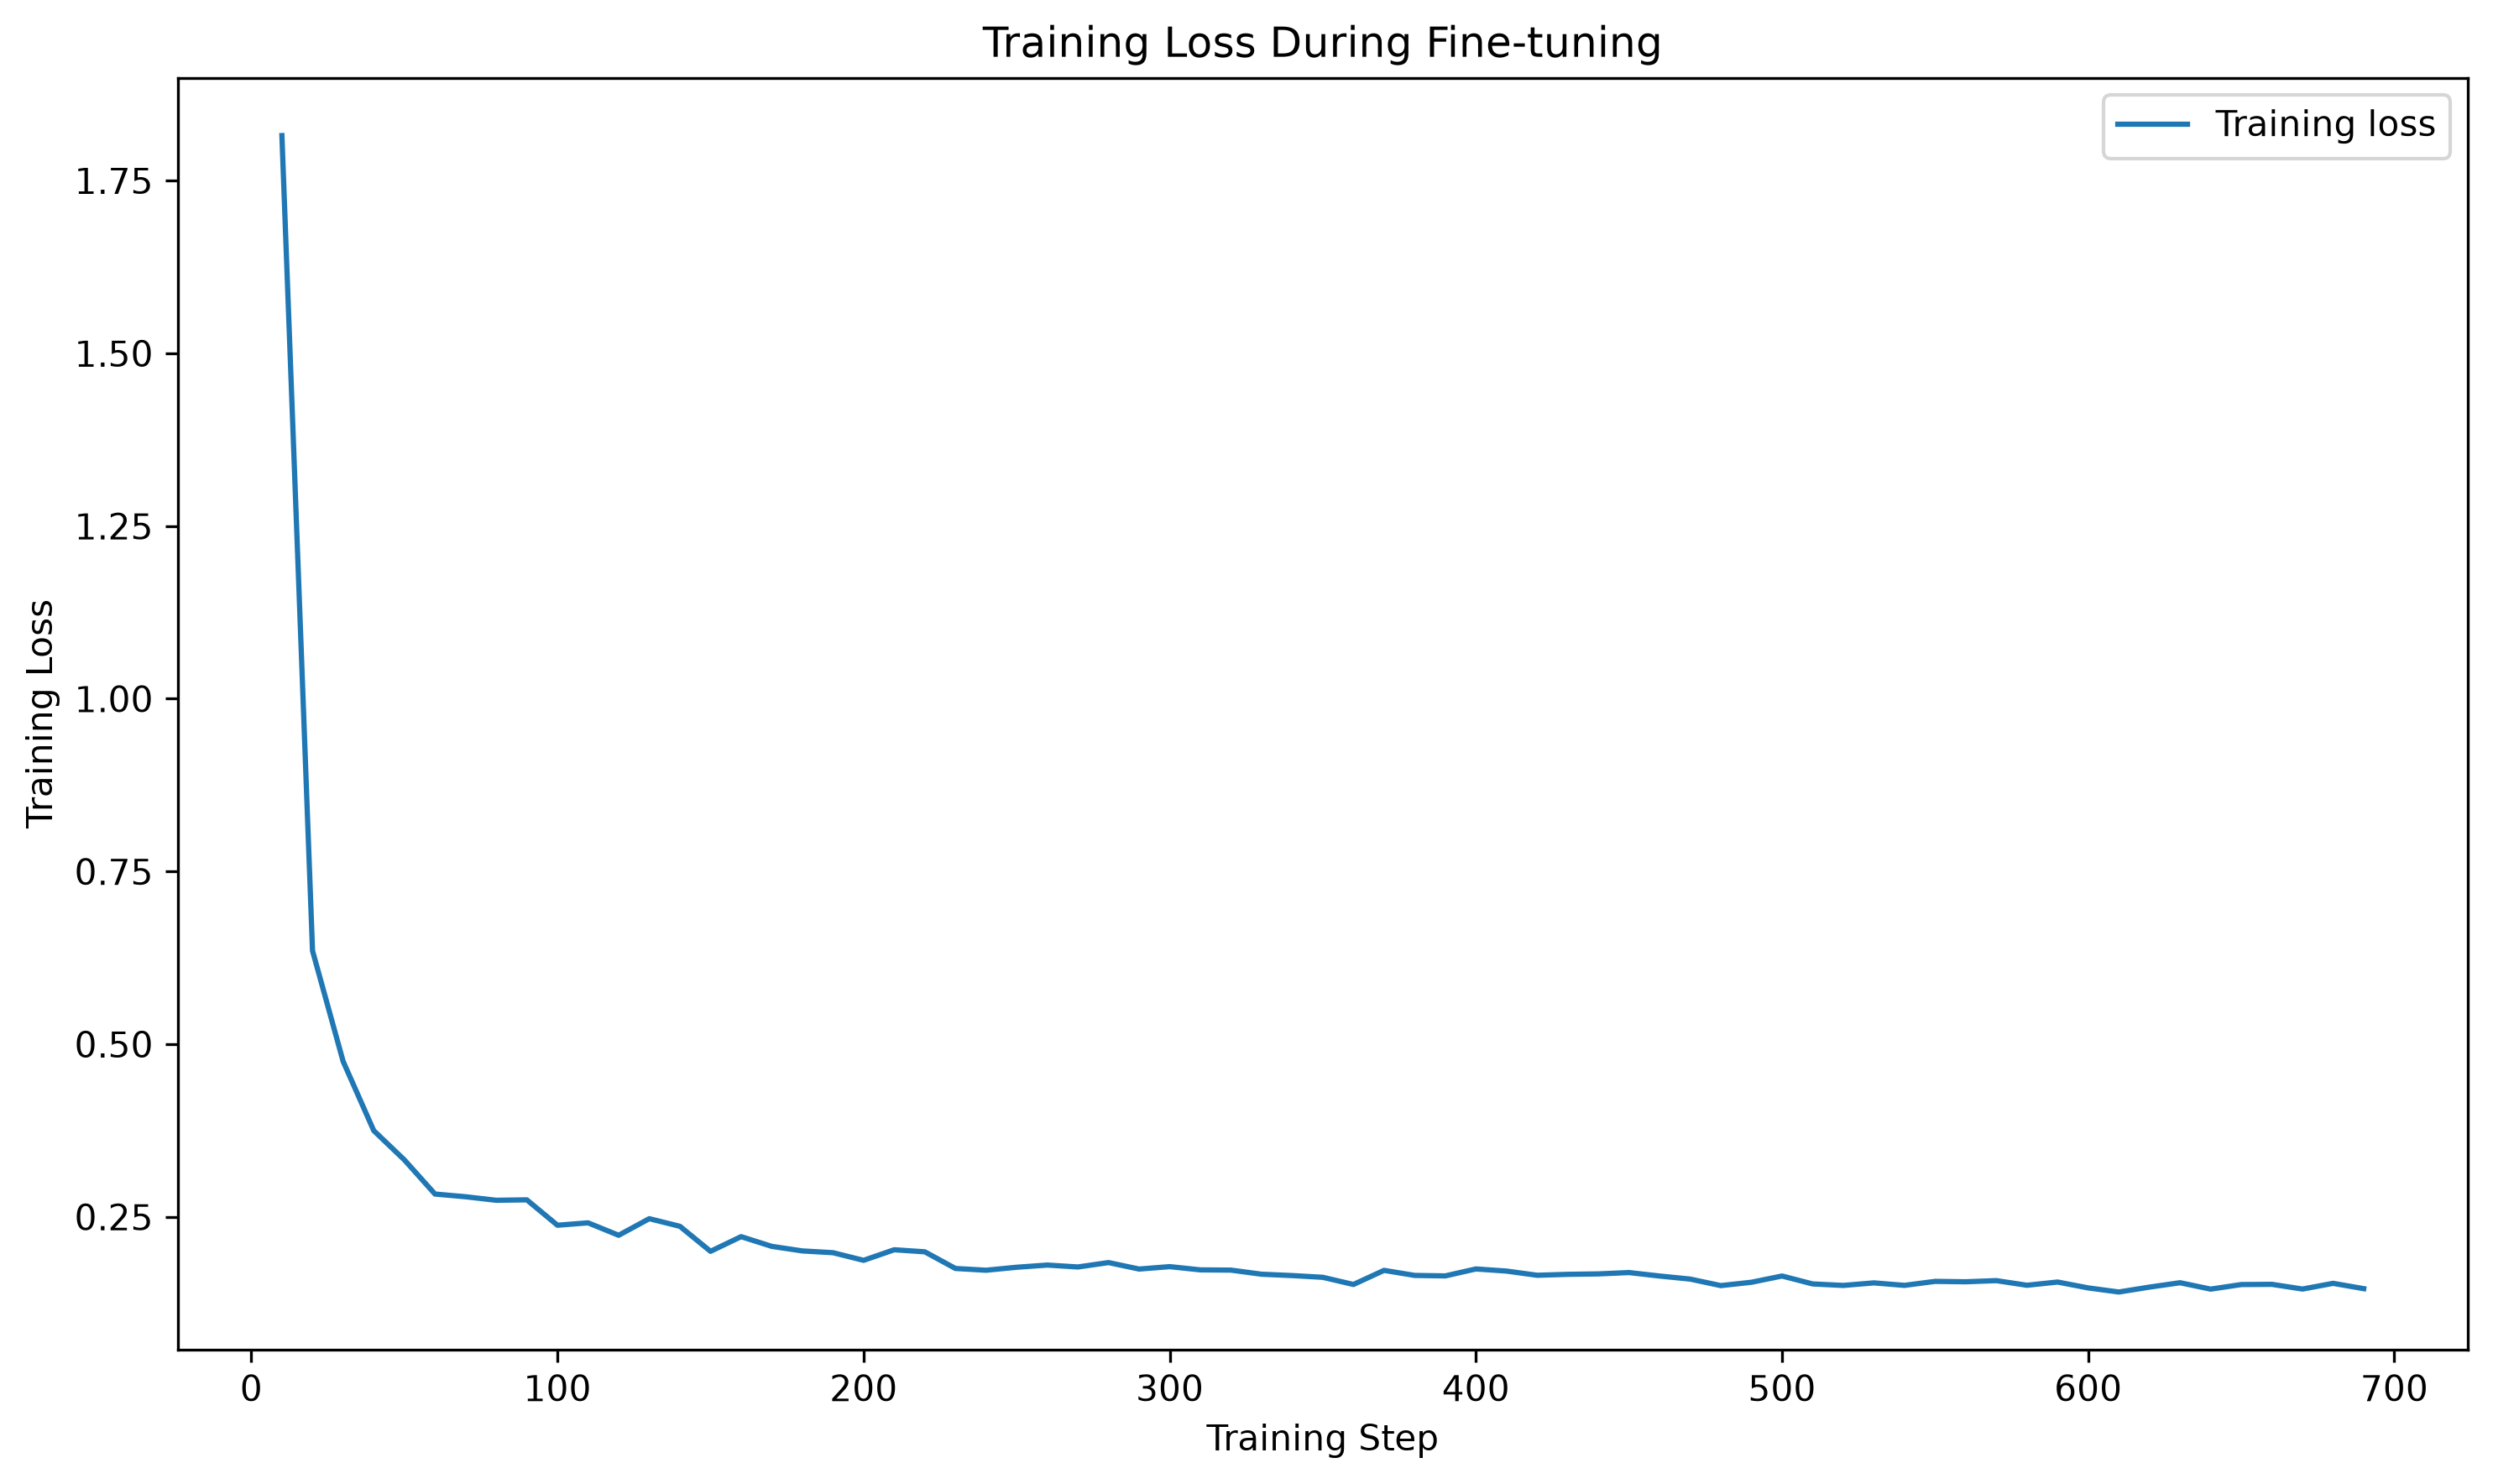
\includegraphics[width=0.9\textwidth]{training_loss.png}
    \caption{Training loss during QLoRA fine-tuning.}
    \label{fig:training_loss}
\end{figure}

Figure 1 shows the training loss recorded during fine-tuning. Loss decreased
rapidly during the early training steps before declining more gradually and
stabilising towards the end of training. This indicates that most of the initial
adaptation occurred early in training, while later steps produced smaller
improvements.


\subsection{Performance by Difficulty Level}

Aggregate accuracy hides substantial variation between translation types. The
first fine-tuned model was therefore evaluated separately by category and
difficulty level.

\begin{table}[ht]
\centering
\caption{Exact-match performance of Fine-Tuned v1 by category.}
\label{tab:v1-category}
\begin{tabular}{lrr}
\toprule
\textbf{Category} & \textbf{Exact Matches} & \textbf{Accuracy} \\
\midrule
Fact                 & 43/53 & 81.13\%  \\
Simple Rule          & 55/60 & 91.67\%  \\
Multi-Condition Rule & 23/45 & 51.11\%  \\
Reasoning            & 41/41 & 100.00\% \\
\bottomrule
\end{tabular}
\end{table}

Simple rules were translated most reliably among the direct translation
categories, reaching 91.67\% exact-match accuracy. Facts achieved 81.13\%.

The most difficult category was Level 3 multi-condition rules. Only 23 of the
45 examples exactly matched the reference, giving an accuracy of 51.11\%.
These examples require the model to maintain several variables and conditions
simultaneously and may include inequality or negation. An error in any
predicate, argument position or condition causes the complete program to fail
exact match.

The Level 4 reasoning examples achieved 100\% exact match in this
category-level analysis, demonstrating that difficulty did not simply increase
monotonically with the assigned level. The Level 4 templates were more
constrained than the range of Level 3 structures, while Level 3 contained
several relational patterns that proved particularly difficult.

This illustrates why reporting only aggregate accuracy would have been
insufficient. An overall exact-match score above 80\% could suggest relatively
uniform performance, while the category analysis shows that the model remained
much less reliable on particular symbolic structures.


\subsection{Error Analysis}

The 37 non-exact predictions from the first fine-tuned model were analysed to
determine whether the failures were random or concentrated in particular
templates.

The most common failure groups are shown in
Table~\ref{tab:v1-errors}.

\begin{table}[ht]
\centering
\caption{Most common non-exact template groups for Fine-Tuned v1.}
\label{tab:v1-errors}
\begin{tabular}{lr}
\toprule
\textbf{Template Group} & \textbf{Non-Exact Predictions} \\
\midrule
\texttt{shared\_child\_inequality} & 10 \\
\texttt{employee\_not\_busy}       & 7  \\
\texttt{binary\_calls}             & 6  \\
\texttt{bird\_not\_flightless}     & 5  \\
\texttt{helps\_same\_direction}    & 5  \\
\texttt{binary\_admires}           & 4  \\
\bottomrule
\end{tabular}
\end{table}

Some examples contributed to more than one diagnostic grouping, so these
counts are useful for identifying recurring patterns rather than as mutually
exclusive error classes.

The \texttt{shared\_child\_inequality} template was particularly problematic.
These examples require several binary relationships to share variables while
also enforcing an inequality condition. Generated programs sometimes reversed
the arguments of a relationship or associated a variable with the wrong
predicate position. The resulting output could remain syntactically valid while
representing a different logical relationship.

Binary predicates were another recurring source of errors. Examples involving
\texttt{calls/2} and \texttt{admires/2} sometimes produced semantically related
but incorrect predicate names. For example, a statement requiring
\texttt{admires} could be represented using a predicate such as
\texttt{respects}. In ordinary natural-language generation, such a substitution
could be considered reasonable. In a formal program, however,
\texttt{admires/2} and \texttt{respects/2} are different predicates unless an
explicit relationship between them has been defined.

Similar errors appeared in negative structures. Templates such as
\texttt{employee\_not\_busy} and \texttt{bird\_not\_flightless} require the
model to preserve negation and the intended predicate simultaneously. A
generated program may be valid Prolog but encode a related concept such as
\texttt{free(X)} instead of the expected logical structure involving
\texttt{\char`\\+ busy(X)}.

These errors demonstrate an important property of the task. Once fine-tuned,
the model rarely failed because it was unable to produce Prolog syntax.
Instead, the remaining failures increasingly concerned the mapping between
natural-language meaning and exact symbolic structure.

Error analysis plays a similar role in related neuro-symbolic research.
Logic-LM uses feedback from the symbolic solver to identify and revise
unsuccessful formalizations. The refinement strategy used in this project
differs because recurring failures were addressed through additional training
examples rather than revising individual outputs during inference.


\subsection{Targeted Refinement Dataset}

The error analysis motivated a second training stage. Rather than increasing
the training set with randomly generated examples, a refinement dataset was
constructed to increase exposure to translation patterns related to the
observed failures.

The refinement dataset contained 250 validated examples. Its distribution is
shown in Table~\ref{tab:refinement-distribution}.

\begin{table}[ht]
\centering
\caption{Distribution of the targeted refinement dataset.}
\label{tab:refinement-distribution}
\begin{tabular}{lr}
\toprule
\textbf{Level} & \textbf{Examples} \\
\midrule
Level 1 & 90  \\
Level 2 & 30  \\
Level 3 & 130 \\
\midrule
\textbf{Total} & \textbf{250} \\
\bottomrule
\end{tabular}
\end{table}

The largest proportion was assigned to Level 3 because this was the weakest
category in the first evaluation. The refinement set included additional
examples involving binary relationships, negation, conjunction and other
structures similar to those appearing frequently in the error analysis.

Examples were validated using the same Prolog validation procedure as the main
dataset before being included in training. The 250 examples were combined with
the original training data, and a second QLoRA adapter was trained. The
validation and test sets were left unchanged.

This design allowed the refinement experiment to test a specific question:
whether additional examples concentrated on known failure patterns could
improve performance without modifying the evaluation set.


\subsection{Refined Model Results}

The refined model, referred to as \textbf{Fine-Tuned v2}, was evaluated using
the same 199 test examples.

The results are shown in Table~\ref{tab:v2-results}.

\begin{table}[ht]
\centering
\caption{Comparison between Fine-Tuned v1 and Fine-Tuned v2.}
\label{tab:v2-results}
\begin{tabular}{lrr}
\toprule
\textbf{Metric} & \textbf{Fine-Tuned v1} & \textbf{Fine-Tuned v2} \\
\midrule
Exact Match       & 81.41\%  & \textbf{87.94\%}  \\
Syntax Valid      & 100.00\% & \textbf{100.00\%} \\
Executable        & 100.00\% & \textbf{100.00\%} \\
Reasoning Correct & 100.00\%  & \textbf{100.00\%} \\
\bottomrule
\end{tabular}
\end{table}

Exact-match accuracy increased from 162 to 175 correct predictions. This
corresponds to an improvement of 6.53 percentage points over the first
fine-tuned model and 87.44 percentage points over the original baseline.
Syntax validity, executability and reasoning correctness remained at 100\%.

All 199 outputs remained syntactically valid and executable. The additional
fine-tuning therefore improved translation accuracy without reducing the
structural reliability achieved by the first model.

Reasoning correctness remained at 41 out of 41 examples. All Level 4
queries therefore continued to produce their expected results under the
refined model.

These final results require an important qualification. The refinement dataset
was constructed after analysing recurring error patterns observed on the
original test set. Although the individual test examples were not directly
included in the refinement training data, information about the structures
and categories on which the first fine-tuned model performed poorly
influenced the second training stage. The Fine-Tuned v2 results should
therefore not be interpreted as performance on a completely untouched
held-out benchmark.

The category-level exact-match results are shown in
Table~\ref{tab:v2-category}.

\begin{table}[ht]
\centering
\caption{Exact-match performance of Fine-Tuned v2 by category.}
\label{tab:v2-category}
\begin{tabular}{lrr}
\toprule
\textbf{Category} & \textbf{Exact Matches} & \textbf{Accuracy} \\
\midrule
Fact                 & 46/53 & 86.79\%  \\
Simple Rule          & 60/60 & 100.00\% \\
Multi-Condition Rule & 28/45 & 62.22\%  \\
Reasoning            & 41/41 & 100.00\% \\
\bottomrule
\end{tabular}
\end{table}

Simple-rule performance increased from 91.67\% to 100\%, while fact
translation increased from 81.13\% to 86.79\%.

Level 3 remained the weakest category, but improved from 51.11\% to 62.22\%.
This is an increase of 11.11 percentage points and represents five additional
exact translations on the 45 Level 3 test examples.

\begin{figure}[htbp]
    \centering
    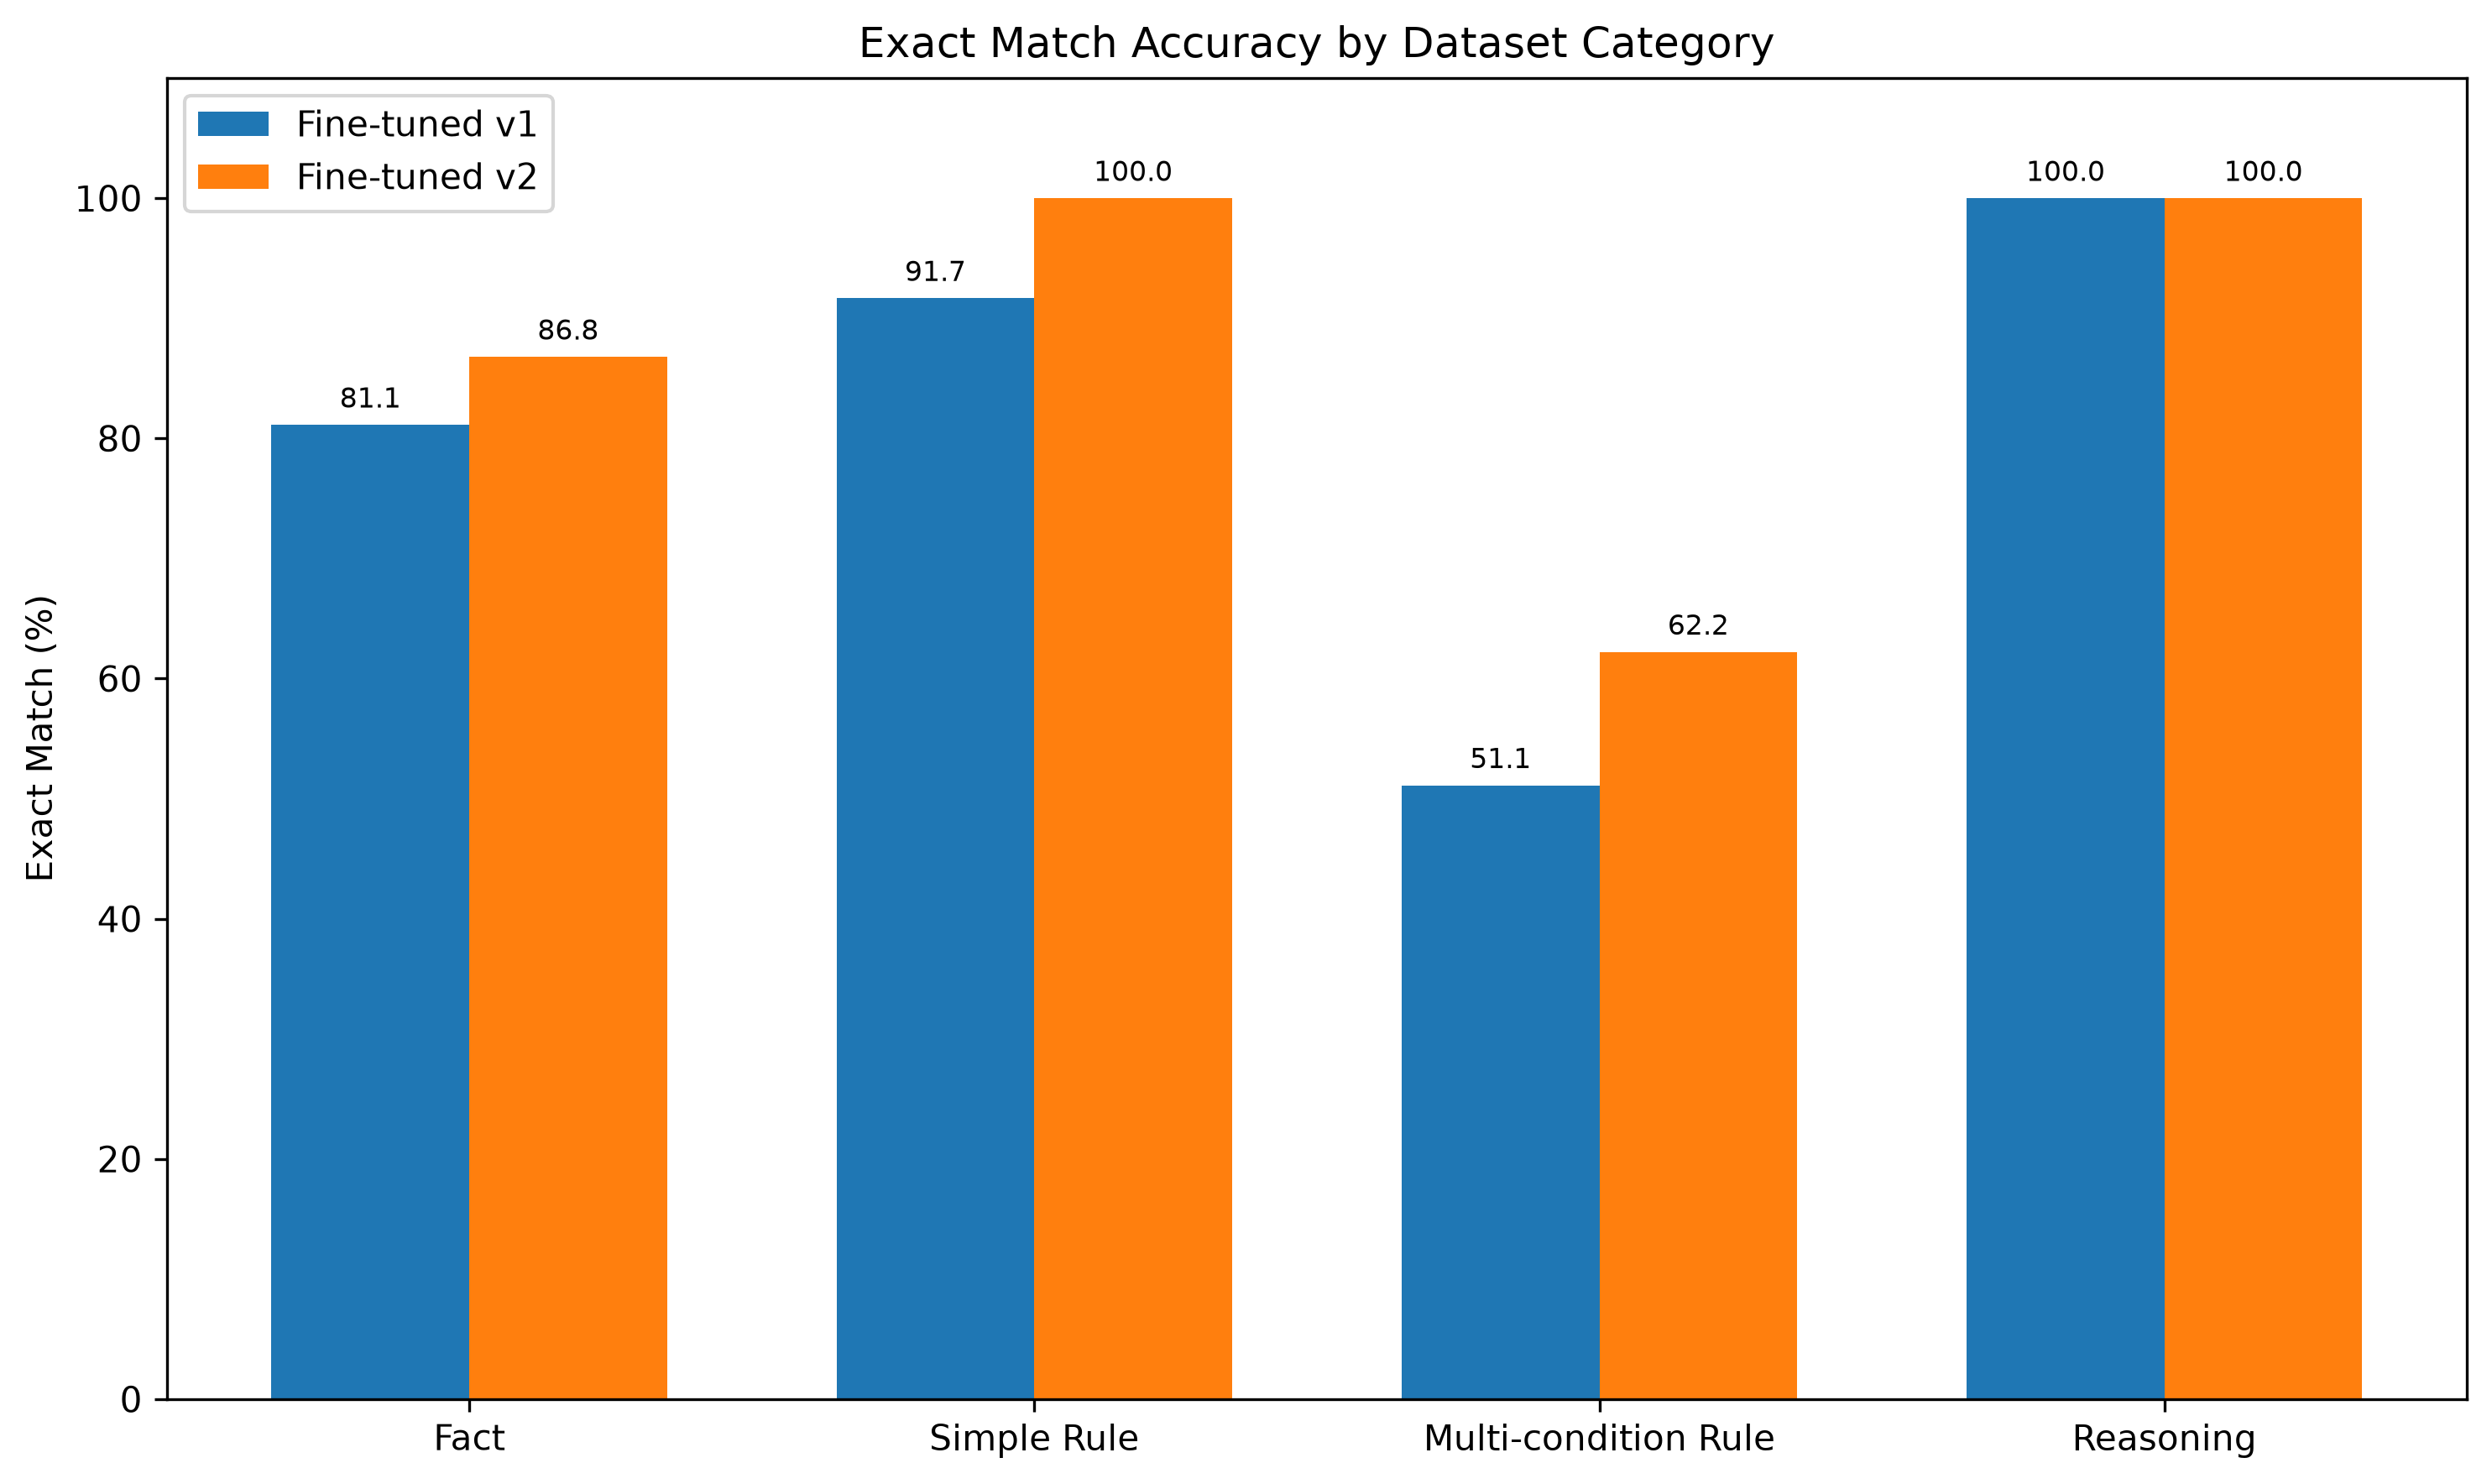
\includegraphics[width=0.9\textwidth]{exact_match_by_category.png}
    \caption{Exact-match accuracy by dataset category for Fine-Tuned v1 and Fine-Tuned v2.}
    \label{fig:category_accuracy}
\end{figure}

Figure 2 provides a direct comparison of exact-match accuracy by category before and after
refinement. The largest improvement occurred for multi-condition rules, although this
category continued to perform substantially below the others. Simple rules reached 100\%,
while reasoning examples remained at 100\% across both fine-tuned versions. The number
of non-exact outputs across the whole test set fell from 37 to 24.


\subsection{Remaining Errors}

Although refinement improved overall performance, several failure patterns
remained.

The most common final failure groups are shown in
Table~\ref{tab:v2-errors}.

\begin{table}[ht]
\centering
\caption{Most common remaining failure groups for Fine-Tuned v2.}
\label{tab:v2-errors}
\begin{tabular}{lr}
\toprule
\textbf{Template Group} & \textbf{Remaining Failures} \\
\midrule
\texttt{shared\_child\_inequality} & 10 \\
\texttt{binary\_admires}           & 4  \\
\texttt{bird\_not\_flightless}     & 4  \\
\texttt{employee\_not\_busy}       & 3  \\
\texttt{binary\_calls}             & 3  \\
\bottomrule
\end{tabular}
\end{table}

The continued presence of all 10
\texttt{shared\_child\_inequality} failures is particularly notable. Unlike
several simpler categories, targeted additional training did not resolve
this structure on the test examples. The pattern combines multiple binary
predicate applications, shared variables and inequality, making errors in
variable binding or argument direction especially consequential.

By contrast, some categories responded strongly to refinement. Simple rules
reached complete exact-match accuracy, and the number of errors involving
several other templates declined. This suggests that targeted additional
examples can correct some systematic translation behaviours, although
different structures respond differently to additional supervision.

\begin{figure}[htbp]
    \centering
    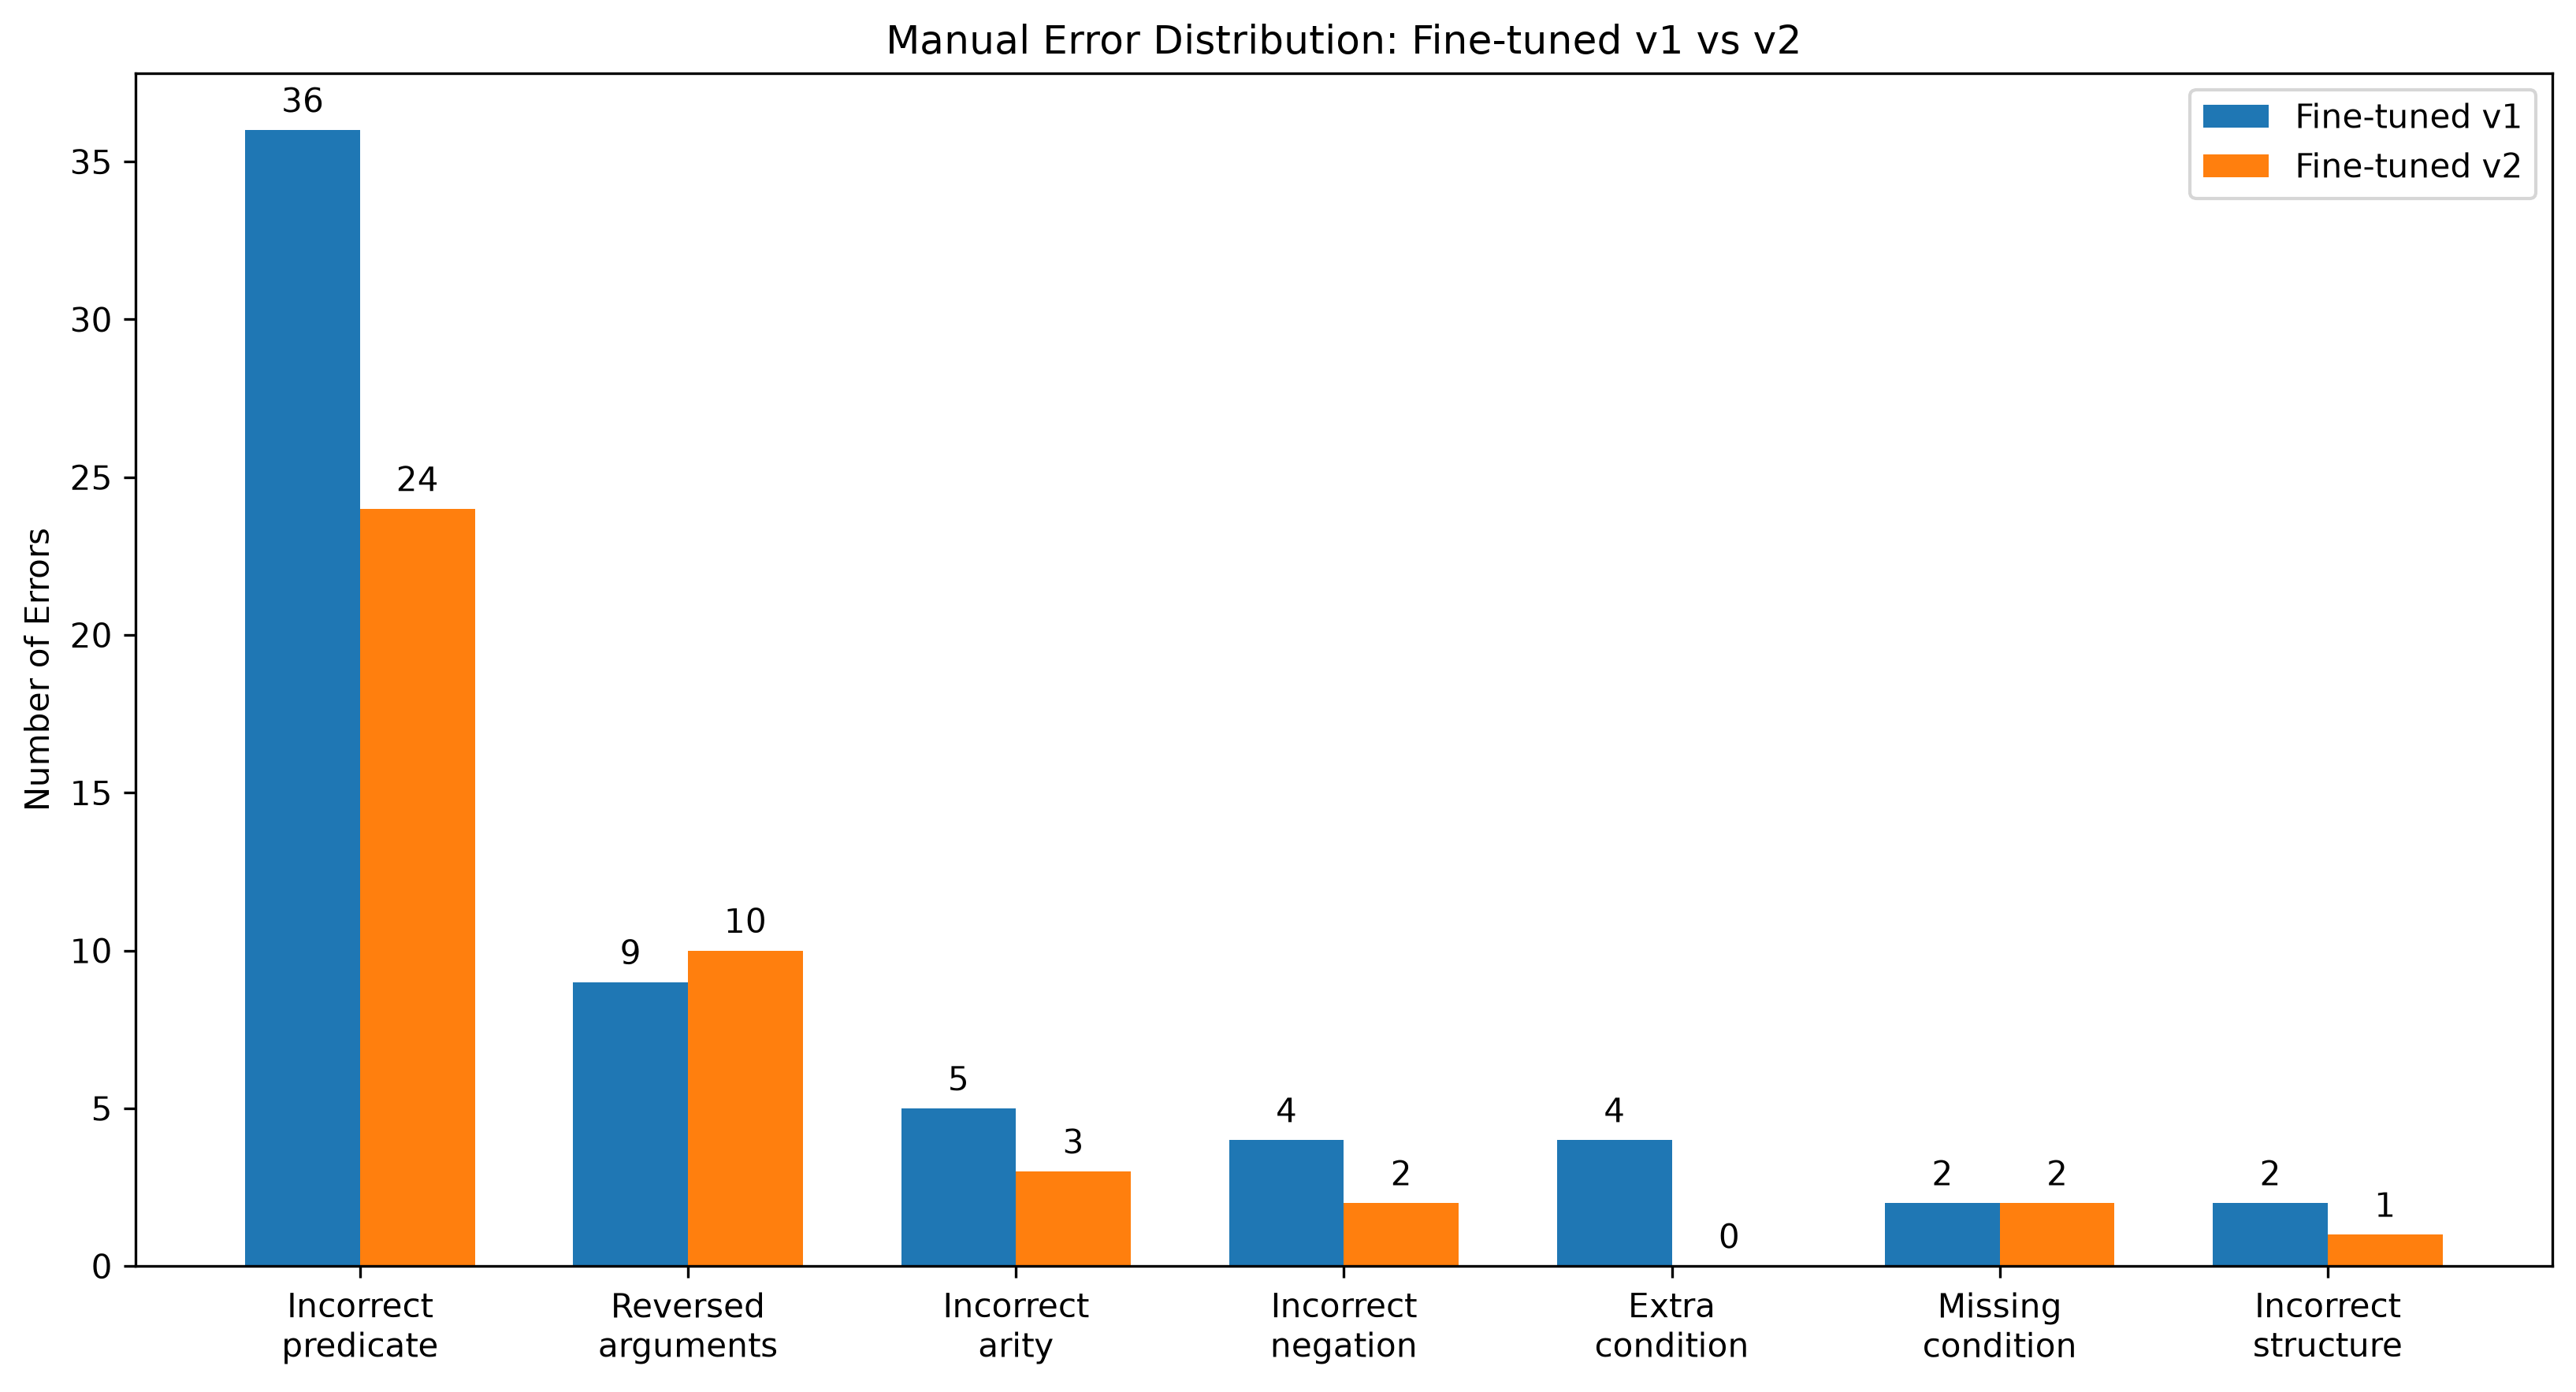
\includegraphics[width=0.95\textwidth]{error_distribution_v1_v2.png}
    \caption{Distribution of manually identified errors for Fine-Tuned v1 and Fine-Tuned v2.}
    \label{fig:error_distribution}
\end{figure}

Figure 3 provides a broader comparison of the manually identified error
types before and after refinement. Incorrect predicate selection remained
the most common error but decreased substantially in the refined model.
Incorrect arity, negation, additional conditions and incorrect structures
also became less frequent. Reversed arguments remained problematic
and increased slightly from nine to ten identified cases. A single prediction
could contain more than one error type, so the counts in the figure do not
sum to the total number of non-exact predictions.

The final 24 non-exact examples also reinforce the distinction between formal
validity and exact semantic translation. Despite these failures, every output
remained syntactically valid and executable. The remaining challenge was
therefore not primarily producing legal Prolog syntax. It was producing the
precise predicates, argument relationships and logical operations specified by
the natural-language input. This indicates that, after fine-tuning, the
dominant source of error had shifted from structural Prolog generation to
semantic alignment between the natural-language input and the generated
symbolic representation.

\subsection{Overall Comparison}

The complete experimental progression is summarised in
Table~\ref{tab:overall-comparison}.

\begin{table}[ht]
\centering
\caption{Overall comparison of the three evaluated model versions.}
\label{tab:overall-comparison}

\small
\setlength{\tabcolsep}{4pt}

\begin{tabular}{lrrrr}
\toprule
\textbf{Model} &
\textbf{Exact Match} &
\textbf{Syntax Valid} &
\textbf{Executable} &
\textbf{Reasoning Correct} \\
\midrule
Baseline      & 0.50\%  & 39.70\%  & 39.70\%  & 14.63\% \\
Fine-Tuned v1 & 81.41\% & 100.00\% & 100.00\% & 100.00\% \\
Fine-Tuned v2 & \textbf{87.94\%} &
                \textbf{100.00\%} &
                \textbf{100.00\%} &
                \textbf{100.00\%} \\
\bottomrule
\end{tabular}
\end{table}

The largest improvement occurred between the baseline and first fine-tuned model,
with exact-match accuracy increasing from 0.50\% to 81.41\%. This indicates that
supervised task-specific adaptation was responsible for the majority of the observed
performance gain. Targeted refinement produced a smaller additional increase from
81.41\% to 87.94\%, suggesting that the second training stage primarily addressed
specific residual weaknesses rather than fundamentally changing the model's
overall translation capability.

\begin{figure}[htbp]
    \centering
    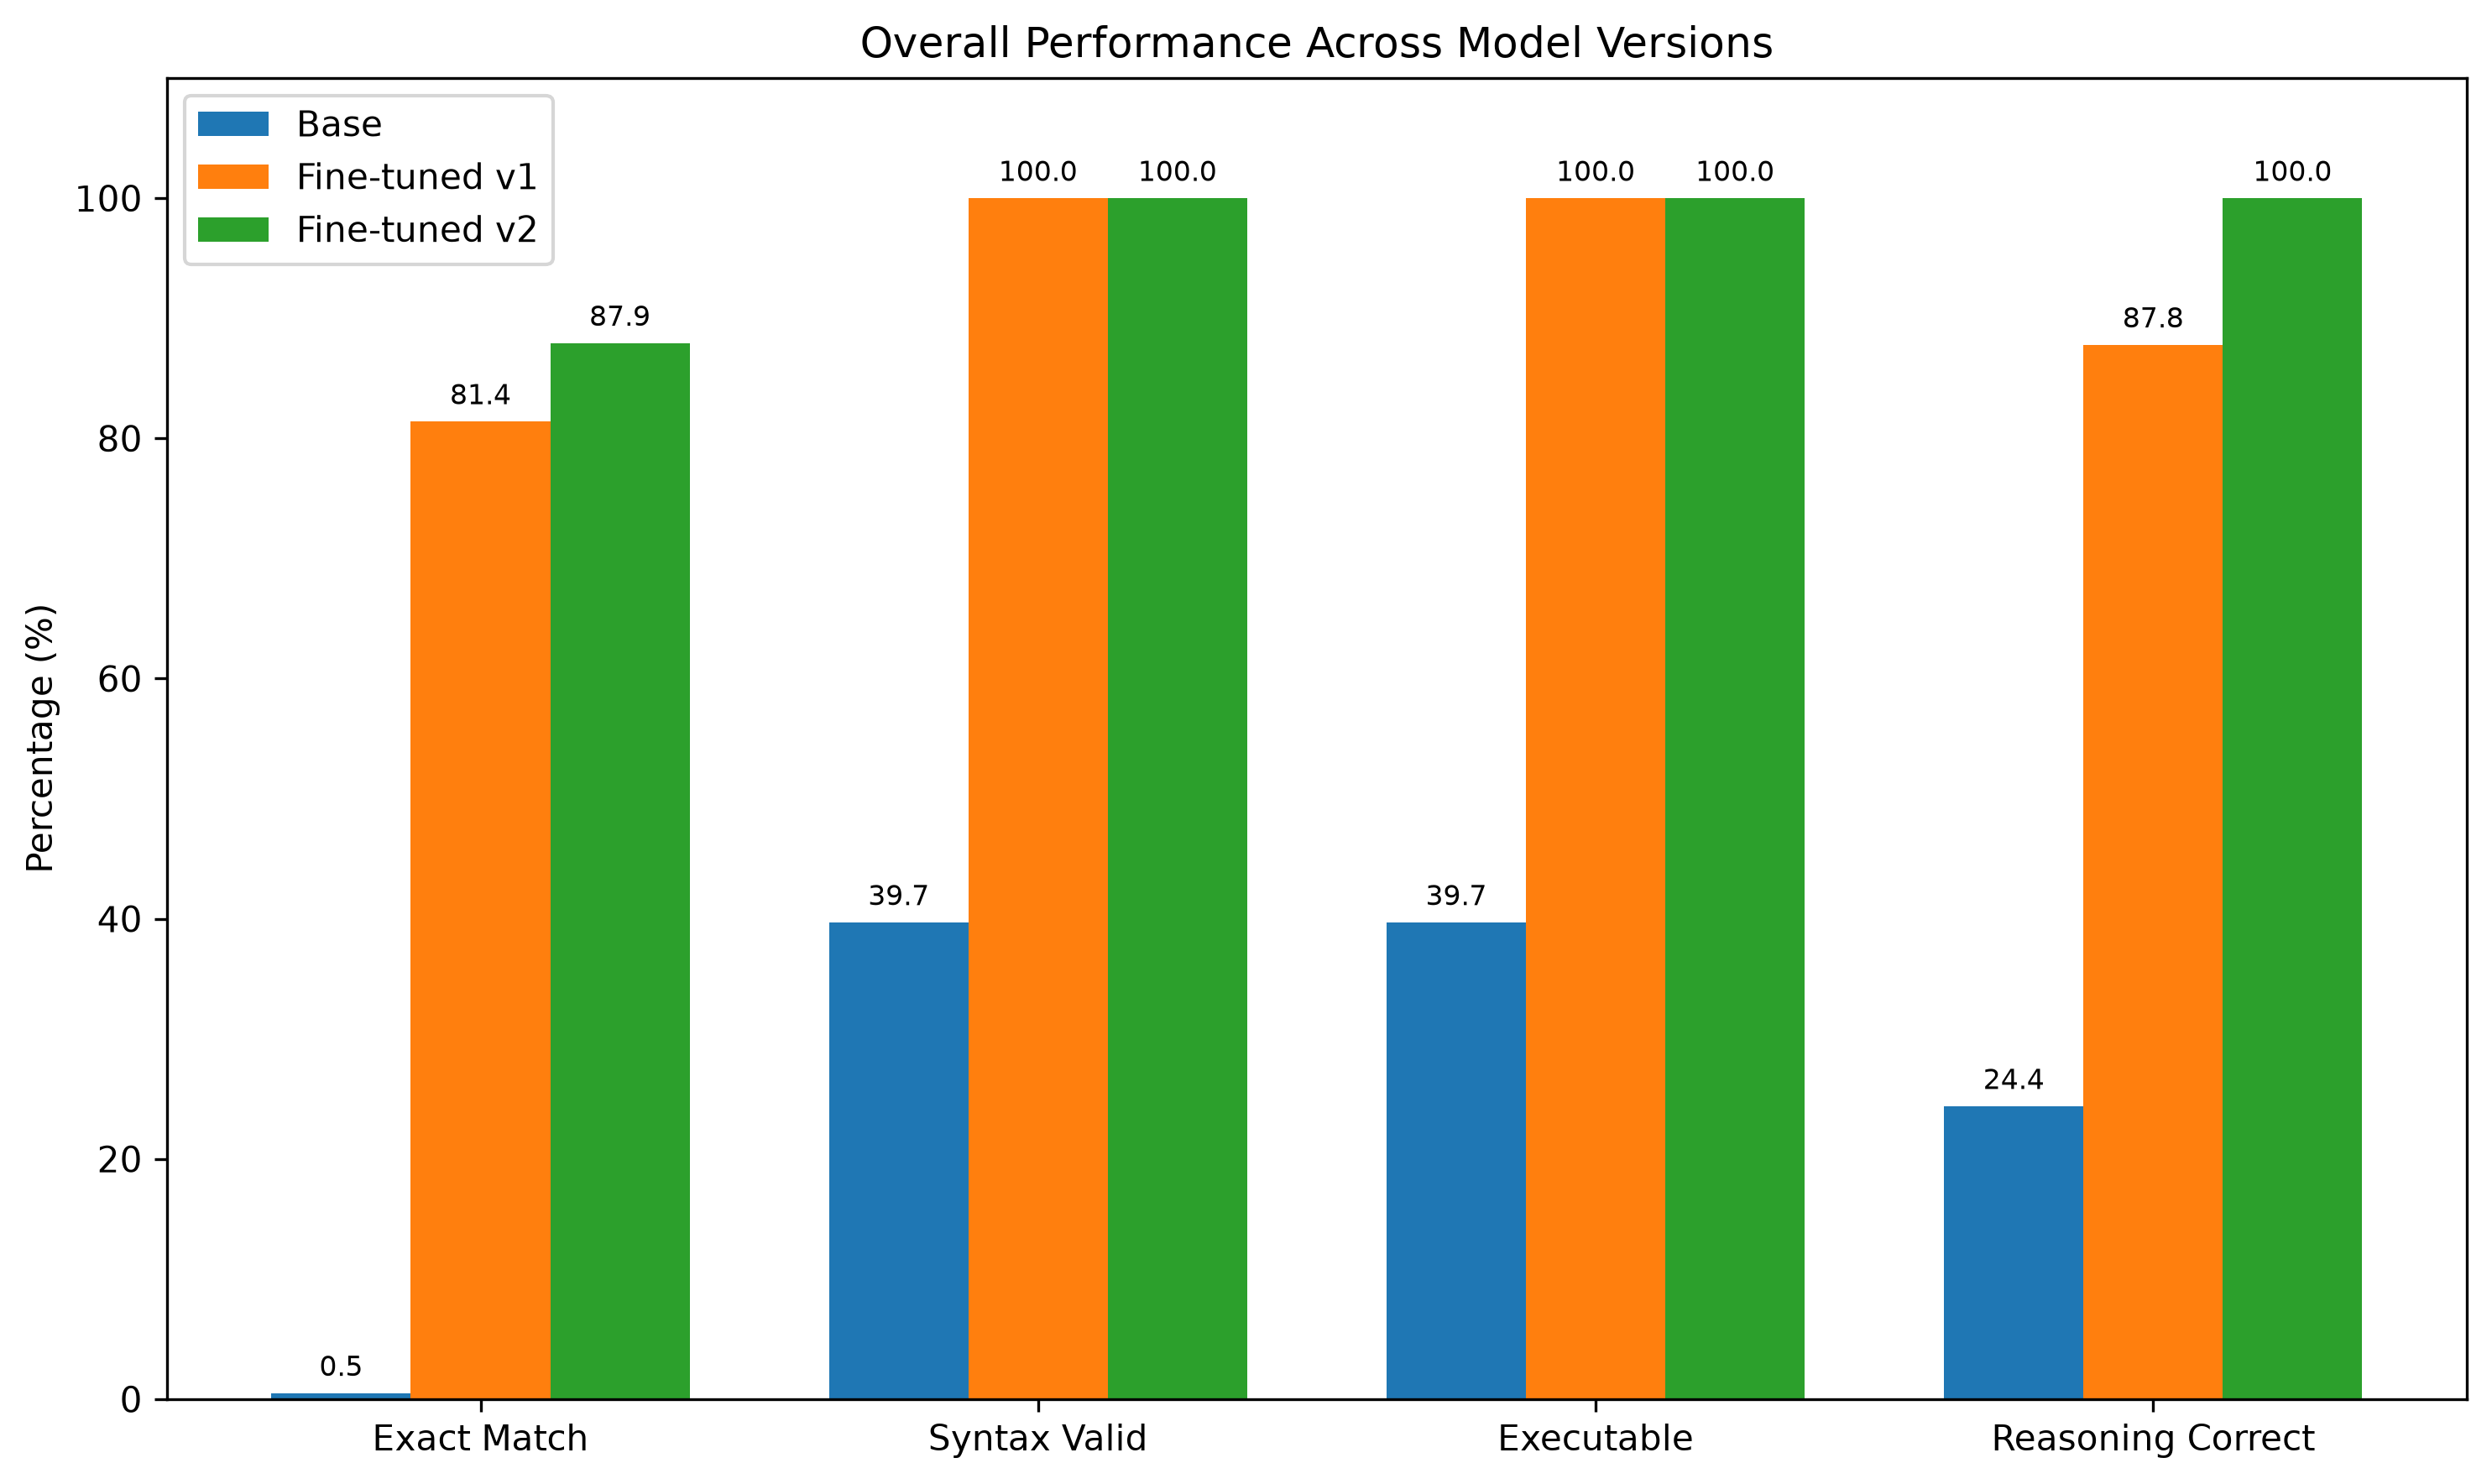
\includegraphics[width=0.95\textwidth]{overall_performance.png}
    \caption{Overall performance of the baseline, Fine-Tuned v1 and Fine-Tuned v2 models.}
    \label{fig:overall_performance}
\end{figure}

Figure 4 visualises the overall progression across the three model versions.
Fine-tuning produced a substantial improvement across all four evaluation
metrics, particularly when compared with the original baseline. The
refinement stage produced a further increase in exact-match accuracy
while maintaining 100\% syntax validity, executability and reasoning correctness.

The results also provide evidence for the usefulness of evaluating symbolic
generation at more than one level. If only syntax validity had been measured,
both fine-tuned models would appear identical at 100\%. Exact-match evaluation
reveals substantial differences between them. Conversely, exact match alone
would not show that all final generations formed executable Prolog programs or
that every reasoning query produced its expected result.

A related motivation appears in LINC, where language models are used as
semantic parsers and external theorem provers perform the deductive reasoning.
This modular approach demonstrates how symbolic execution can complement neural
language processing, provided that the intermediate formalization is
sufficiently accurate.

The experiments in this project examine the preceding problem more directly:
whether a small language model can be trained to produce that intermediate
symbolic representation reliably. The progression from 0.50\% to 87.94\%
exact match, together with complete syntactic validity and executability in the
final model, shows that Qwen2.5-1.5B can acquire strong NL to Prolog translation
behaviour from a relatively small, controlled dataset. At the same time, the
remaining Level 3 failures show that syntactically correct generation does not
guarantee precise semantic formalization. The implications and limitations of
these findings are considered in Chapter 6.

% ============================================================
\clearpage
\section{Discussion}
% ============================================================

The experiments demonstrate that a small language model can be adapted to
perform natural-language-to-Prolog translation with substantially greater
reliability than the original instruction-tuned model. Fine-tuning
Qwen2.5-1.5B-Instruct increased exact-match accuracy from 0.50\% to 81.41\%,
while targeted refinement increased this further to 87.94\%. Both fine-tuned
models also generated syntactically valid and executable Prolog for every
example in the test set. These results answer the central research question
positively within the controlled setting of this project: a
1.5-billion-parameter language model can learn a strong mapping from
natural-language reasoning statements to executable Prolog through
task-specific training.

However, the different evaluation metrics and remaining errors show that this
conclusion requires qualification. The model learned Prolog syntax more
completely than it learned the exact semantic mappings represented in the
dataset. The results also depend on a synthetic and relatively constrained
dataset, and the refinement procedure introduces limitations in how the final
test performance should be interpreted.


\subsection{Effect of Fine-Tuning}

The largest improvement occurred between the baseline and the first fine-tuned
model. Exact match increased by more than 80 percentage points, while syntax
validity and executability both increased from 39.70\% to 100\%. This suggests
that task-specific supervision was much more important than the model's
existing general ability to generate code.

The baseline demonstrates that instruction tuning alone was insufficient for
this specialised task. Qwen2.5-1.5B-Instruct occasionally generated valid
Prolog-like output, but it rarely produced the expected formal representation.
After being exposed to 1,597 paired examples, the model consistently followed
the required syntax and usually mapped the natural-language input to the
expected predicates and rules.

This supports the broader principle behind parameter-efficient adaptation.
QLoRA was originally proposed as a way of adapting quantised language models
while reducing the memory required for training. In this project, it allowed
task-specific behaviour to be learned using a consumer GPU rather than
requiring full-parameter training. The result is significant for the aim of
the project because it suggests that useful autoformalization behaviour is not
restricted to very large models or high-resource training environments.

The result should not, however, be interpreted as showing that a 1.5B model
has acquired general natural-language-to-Prolog translation ability. The
training and evaluation language is deliberately constrained. The stronger
conclusion supported by the experiments is that a small model can learn this
mapping effectively within a controlled domain.


\subsection{Symbolic Execution as an Evaluation Tool}

One of the clearest findings is the value of evaluating generated
formalizations at more than one level. Exact match, syntax validity,
executability and reasoning correctness measure related but different
properties.

The final model achieved 87.94\% exact match while achieving 100\% syntax
validity and executability. Therefore, 24 outputs differed from the reference
despite still forming legal Prolog programs. This distinction would have been
hidden if only a single metric had been used.

Execution-based evaluation is particularly appropriate for formal outputs
because it takes advantage of information that is unavailable when evaluating
unrestricted natural language. Previous work on natural-language-to-code
translation has similarly demonstrated that program execution can provide
useful semantic information beyond execution-unaware comparison \cite{shi2022execution}. Candidate
programs can, for example, be distinguished according to their execution
behaviour rather than assuming that surface similarity alone determines
correctness.

The findings of this project support the same general principle. An exact
textual comparison is useful because the dataset defines a specific intended
representation, but it is strict. Two programs may differ textually while
remaining executable. At the same time, executability alone is too weak: a
program can execute successfully while representing the wrong relationship.

The remaining errors demonstrate this directly. Generating
\texttt{respects(X,Y)} instead of \texttt{admires(X,Y)} may produce perfectly
valid Prolog, yet the symbolic meaning differs from the reference. Similarly,
reversing arguments in \texttt{parent/2} produces a syntactically valid program
representing a different relationship. Therefore, execution should complement
rather than replace semantic evaluation.

\subsection{Reasoning Correctness}

Reasoning accuracy showed one of the largest improvements between the baseline
and fine-tuned models, increasing from 14.63\% for the baseline to 100\% for
the first fine-tuned model and remaining at 100\% for the refined model. This
provides evidence that the generated programs were not merely syntactically
well formed. For the 41 reasoning examples in the final test set, every program
generated by both fine-tuned models supported the expected query result.

This result is consistent with the motivation of neuro-symbolic approaches
such as Logic-LM and LINC. Logic-LM separates translation from inference by
having a language model create a symbolic formulation before a deterministic
solver performs reasoning. LINC similarly treats the language model as a
semantic parser and delegates deduction to a first-order logic prover.

The present system follows the same broad separation but focuses on improving
the translation stage through fine-tuning. Once a correct Prolog
representation has been generated, SWI-Prolog can perform the inference
deterministically.

Nevertheless, 100\% reasoning accuracy should not be interpreted as evidence
that the model can solve arbitrary logical problems. Only 41 reasoning examples
from the test set were evaluated, and they originated from the controlled
Level 4 templates used by the project. The result demonstrates complete
performance on this test subset rather than universal reasoning capability.


\subsection{Remaining Difficulties}

The distribution of errors reveals that formalization difficulty depends
strongly on logical structure. Simple rules achieved 100\% exact match in the
refined model, while multi-condition rules reached only 62.22\%.

The persistent \texttt{shared\_child\_inequality} failures are particularly
informative. These examples require the model to maintain several predicates,
variable relationships and an inequality constraint simultaneously. All ten
examples in this failure group remained incorrect after refinement. This
suggests that adding more examples alone did not completely solve the
underlying structural problem.

Errors involving binary predicates reveal another challenge. Natural language
allows concepts such as ``admires'' and ``respects'' to be treated as
semantically related. Formal programming languages do not provide this
flexibility unless that relationship has been explicitly defined.
Autoformalization therefore requires a model to suppress some of its normal
linguistic behaviour and preserve exact predicate identity.

This supports an observation made in related neuro-symbolic work: the
semantic-parsing stage remains a major failure point even when a symbolic
prover can perform deduction reliably. The symbolic component removes
uncertainty from the inference stage, but it cannot correct a program that
encodes the wrong meaning.

Recent work using Prolog provides a further comparison. Research involving
language models using Prolog as an external reasoning tool has highlighted a
distinction between answer accuracy and the production of fully auditable
symbolic programs. Obtaining a correct answer does not necessarily mean that
the intermediate symbolic representation is itself faithful. This reinforces
the decision in the present project to evaluate the generated Prolog directly
rather than judging only the final reasoning result.


\subsection{Effect of Targeted Refinement}

The refinement experiment increased exact-match accuracy from 81.41\% to
87.94\%, reduced non-exact outputs from 37 to 24 while reasoning
correctness remained at 100\%. The improvement indicates that error analysis
can be used to guide additional training more efficiently than simply
generating more examples without considering model behaviour.

This is conceptually related to approaches that use symbolic-solver feedback
to improve failed formalizations. The mechanism used here differs: instead of
revising a failed output during inference, recurring errors were identified
across the evaluation results and used to construct new supervised training
examples.

However, this refinement procedure also creates an important limitation. The
errors used to decide which examples required additional training were observed
on the same test set later used to report the Fine-Tuned v2 results. Although
the exact test examples themselves were not added to the training set,
information about their failure categories influenced the refinement data. The
v2 test set was therefore no longer completely independent of model
development.

Consequently, the 87.94\% final exact-match result should be interpreted
primarily as evidence that targeted refinement improved performance on the
identified weaknesses. A stronger estimate of final generalisation would
require a second untouched test set that was not inspected until all refinement
decisions had been completed. Future work should use the validation or
development set for error-driven refinement and reserve an independent final
test set solely for the last evaluation.


\subsection{Dataset and Experimental Limitations}

The primary limitation of the project is the controlled nature of the dataset.
Synthetic generation made it possible to know the intended Prolog
representation, automatically validate every target and systematically vary
logical structures. However, the resulting natural language is less diverse
than unrestricted human writing.

The model may therefore have learned recurring correspondences between
templates and Prolog structures rather than developing a general ability to
formalize arbitrary natural language. Group-aware splitting reduces direct
leakage between related template examples, but it cannot completely reproduce
the variation found in naturally written reasoning problems.

The test set is also relatively small at 199 examples. Category-level results
are therefore based on much smaller subsets, including only 45 multi-condition
rules and 41 reasoning examples. Additional evaluation on independently
written examples, external datasets or deliberately adversarial paraphrases
would provide stronger evidence about generalisation.

A further limitation is the loss of test-set independence during targeted refinement.
As discussed above, the test examples themselves were not added to the
refinement dataset, but their observed failure patterns influenced its construction.
The refined-model results may therefore provide an optimistic estimate of
performance compared with evaluation on a completely unseen dataset.

Only one base model size and one main training configuration were also
evaluated. The experiments therefore cannot determine whether
Qwen2.5-1.5B-Instruct is optimal, how performance scales with model size, or
whether different LoRA parameters, training durations or dataset sizes would
produce better results. These questions were outside the practical scope of
the project but provide clear directions for further work.

Overall, the experiments demonstrate that fine-tuning can make a small
language model highly reliable at generating executable Prolog within a
controlled domain. They also show why symbolic validation is valuable:
Prolog execution makes structural failures directly observable and supports
functional reasoning tests. The remaining errors, particularly in
multi-condition relations, indicate that the more difficult problem is not
learning Prolog syntax but preserving precise semantics when translating
increasingly complex natural-language structures.

% ============================================================
\clearpage
\section{Conclusion and Future Work}
% ============================================================

This project investigated whether a small language model could be trained to
translate natural-language reasoning statements into executable Prolog. The
motivation was to explore autoformalization as a way of combining the
natural-language capabilities of language models with the explicit and
verifiable reasoning provided by symbolic systems. Rather than relying on a
language model to perform both interpretation and reasoning internally, the
developed system uses the model to generate a formal Prolog representation
that can subsequently be checked and executed using SWI-Prolog.

A controlled dataset of 2,000 natural-language and Prolog pairs was constructed
for this purpose. The examples were divided into four levels covering facts,
simple rules, multi-condition rules and reasoning problems. Automated
validation with SWI-Prolog ensured that all target programs were syntactically
valid and executable, while reasoning examples were additionally checked
against their expected query results. A group-aware training, validation and
test split was used to reduce direct leakage between closely related generated
templates.

The experiments used Qwen2.5-1.5B-Instruct as the base model. Before
fine-tuning, its performance on the 199-example test set was poor. Exact-match
accuracy was only 0.50\%, while 39.70\% of outputs were syntactically valid and
executable. Reasoning correctness was 14.63\%. The poor baseline performance
indicates that general instruction-following ability alone was insufficient for
reliable natural-language-to-Prolog translation.


QLoRA fine-tuning produced a substantial improvement. The first fine-tuned
model achieved 81.41\% exact-match accuracy, while every generated program was
syntactically valid and executable. Reasoning accuracy increased to 100\%.
Error analysis showed that the remaining failures were concentrated in
particular structures rather than being evenly distributed across the dataset.
Multi-condition rules were especially difficult, with recurring errors
involving binary predicate direction, inequality and negation.

These observations were used to construct an additional refinement dataset
containing 250 targeted examples. Following a second training stage,
exact-match accuracy increased to 87.94\%. Syntax validity and executability
remained at 100\%, while all 41 reasoning examples produced their expected
results. Simple-rule exact match reached 100\%, although multi-condition rules
remained the weakest category at 62.22\%. This suggests that the model learned
the basic syntax and structure of Prolog more reliably than some of the more
complex semantic relationships expressed within it.

The results therefore provide a positive answer to the central research
question within the scope of the experiment. A 1.5-billion-parameter language
model can be fine-tuned to perform NL to Prolog autoformalization with high
reliability on a controlled domain, and parameter-efficient training makes
this possible using consumer hardware. Prolog execution also proved useful
as an evaluation mechanism. Exact match alone does not fully describe model
performance: an output can differ from the reference while remaining
executable, while an executable program may still encode an incorrect semantic
relationship. Combining exact match with syntax, execution and reasoning
evaluation therefore gives a more informative picture of autoformalization
quality.

There are several limitations to these conclusions. The dataset was synthetically
generated from controlled templates and consequently does not represent the
full linguistic variation of naturally written reasoning problems. The test set was
also relatively small. As discussed in the previous section, the targeted
refinement procedure additionally limits the independence of the final
refined-model evaluation.


Future work should therefore evaluate the model on natural or independently
written language, including paraphrases and structures not represented by the
original templates. A stronger experimental design could use a development set
for error-driven refinement while reserving a second test set until all model
development is complete. Further experiments could also compare different
model sizes, training-set sizes and parameter-efficient fine-tuning
configurations.

The most persistent Level 3 errors provide another direction for future
research. Additional work could investigate more structured training for
variable bindings and argument ordering, or use feedback from SWI-Prolog
during generation and refinement rather than only after prediction. A system
could, for example, detect invalid or unsuccessful generated programs and
request a corrected formalization automatically. This would extend the current
pipeline from execution-based evaluation towards execution-guided generation.

Overall, the findings show that relatively small language models can learn a
useful interface between natural language and symbolic logic. Although the
resulting model is not a general-purpose autoformalizer, the substantial
improvement over the untuned baseline and the reliability of the executable
output support task-specific language-model training combined with symbolic
validation as a practical approach to producing more checkable forms of
machine reasoning.


% ============================================================
\clearpage
\section{How to Use My Project}
\label{sec:code-usage}
% ============================================================

The source code accompanying this dissertation is provided in the project
submission directory. It contains the scripts used to generate and validate
the dataset, create the dataset splits, run model inference, fine-tune
Qwen2.5-1.5B-Instruct using QLoRA, and evaluate the resulting models.

This section provides instructions for reproducing the main experimental
pipeline.

All commands below should be executed from the root directory of the submitted
project source code.


\subsection{Requirements}

The project was developed using Python and SWI-Prolog. The required Python
packages and their versions are provided in \path{requirements.txt}.

A CUDA-compatible NVIDIA GPU is required for fine-tuning with the submitted
training script and is recommended for model inference, while SWI-Prolog must
be installed separately and accessible through the \texttt{swipl} command.

After extracting the submitted project files, open a terminal in the project
root directory.

\begin{lstlisting}
python -m venv .venv
\end{lstlisting}

On Windows PowerShell, the environment can be activated using:

\begin{lstlisting}
.venv\Scripts\Activate.ps1
\end{lstlisting}

On Linux or macOS, it can instead be activated using:

\begin{lstlisting}
source .venv/bin/activate
\end{lstlisting}

The required Python packages can then be installed using:

\begin{lstlisting}
pip install -r requirements.txt
\end{lstlisting}

SWI-Prolog must also be installed before running dataset validation or
evaluation. Its installation can be checked using:

\begin{lstlisting}
swipl --version
\end{lstlisting}

All project scripts must be run inside the virtual environment.

\subsection{Dataset Generation and Validation}

The original NL to Prolog dataset can be generated from the project root using:

\begin{lstlisting}
python src/dataset/generate_dataset.py
\end{lstlisting}

This generates the natural-language and Prolog pairs used by the project,
including their level, category and template-group metadata.

The generated examples can then be validated using SWI-Prolog with:

\begin{lstlisting}
python src/evaluation/validate_dataset.py
\end{lstlisting}

The validation procedure checks whether the target Prolog programs are
syntactically valid and executable. For reasoning examples, the associated
query is additionally executed and compared with its expected result.

After validation, the dataset can be divided into training, validation and
test sets using:

\begin{lstlisting}
python src/dataset/split_dataset.py
\end{lstlisting}

The splitting procedure uses the fixed random seed \texttt{4242564} and
assigns examples according to their template groups. This produces the fixed
training, validation and test splits used in the experiments described in
Chapters 4 and 5.


\subsection{Baseline Inference}

Baseline predictions are generated using the original
Qwen2.5-1.5B-Instruct model without task-specific fine-tuning. Baseline
inference can be run using:

\begin{lstlisting}
python src/inference/run_baseline.py
\end{lstlisting}

The model is instructed to return only Prolog code for each natural-language
input. Generated predictions are stored under the baseline results directory
for subsequent evaluation.


\subsection{Model Fine-Tuning}

Model fine-tuning is performed using:

\begin{lstlisting}
python src/training/fine_tune.py
\end{lstlisting}

The training script loads Qwen2.5-1.5B-Instruct using 4-bit NF4
quantisation and trains LoRA adapters using QLoRA. The experiments use three
training epochs, a per-device batch size of two, gradient accumulation over
four steps, a learning rate of $2\times10^{-4}$ and the random seed
\texttt{4242564}, as described in Chapter 4.

The submitted version of \path{src/training/fine_tune.py} is configured for
the final refined experiment and therefore uses
\path{dataset/splits/train_v2.jsonl} as its training dataset. The resulting
adapter is saved to:

\begin{lstlisting}
models/qwen2.5-1.5b-prolog-lora-v2
\end{lstlisting}

To reproduce the initial fine-tuned model, the constants at the beginning of
\path{src/training/fine_tune.py} should instead be set to:

\begin{lstlisting}
TRAIN_PATH = Path("dataset/splits/train.jsonl")
OUTPUT_DIR = Path("models/qwen2.5-1.5b-prolog-lora")
\end{lstlisting}

The LoRA adapters are stored separately from the original Qwen model, allowing
the base model and each fine-tuned version to be evaluated independently.


\subsection{Refinement Dataset and Second Training Stage}

Following evaluation of the first fine-tuned model, the targeted refinement
dataset used in the second training stage can be generated using:

\begin{lstlisting}
python src/dataset/generate_refinement_v2.py
\end{lstlisting}

This produces the additional 250 examples designed to increase representation
of structures associated with recurring errors in the first fine-tuned model.

The refinement examples can then be validated using:

\begin{lstlisting}
python src/dataset/validate_refinement_v2.py
\end{lstlisting}

The validated refinement examples are combined with the original training
split to construct the second-stage training dataset using:

\begin{lstlisting}
python src/dataset/build_train_v2.py
\end{lstlisting}

This produces \path{dataset/splits/train_v2.jsonl}. The submitted
\path{src/training/fine_tune.py} script is configured to use this file and
save the refined adapter separately from the first fine-tuned model.

As discussed in Chapters 5 and 6, the refinement data were designed after
examining error patterns on the test set. The resulting refined-model
evaluation should therefore not be interpreted as evaluation on a completely
untouched test set.


\subsection{Evaluation}

Generated predictions can be evaluated using:

\begin{lstlisting}
python src/evaluation/evaluate_predictions.py
\end{lstlisting}

The evaluation procedure compares each prediction with its reference output
and calculates exact-match accuracy. SWI-Prolog is additionally used to
determine whether generated programs are syntactically valid and executable.

For Level 4 reasoning examples, the associated query is executed against the
generated program and its result is compared with the expected result. This
produces the four principal evaluation measures used in the dissertation:
exact match, syntax validity, executability and reasoning correctness.

Detailed prediction-level results and aggregate metrics are stored in the
corresponding subdirectories of \path{results/}.


\subsection{Error Analysis}

Errors in the generated predictions can be analysed using the project's error
analysis script:

\begin{lstlisting}
python src/evaluation/analyse_errors.py
\end{lstlisting}

The analysis identifies non-exact predictions and groups performance according
to properties such as dataset category, difficulty level and template group.
These results were used to identify recurring translation weaknesses and to
guide construction of the refinement dataset described in Chapter 5.


\subsection{Reproducing the Experimental Workflow}

To reproduce the main experimental procedure described in this dissertation,
the scripts should be executed in the following order:

\begin{enumerate}

    \item Generate the original dataset using
    \path{src/dataset/generate_dataset.py}.

    \item Validate the generated examples using SWI-Prolog with
    \path{src/evaluation/validate_dataset.py}.

    \item Create the fixed training, validation and test splits using
    \path{src/dataset/split_dataset.py}.

    \item Generate predictions from the untuned baseline model using
    \path{src/inference/run_baseline.py}.

    \item Evaluate the baseline predictions using
    \path{src/evaluation/evaluate_predictions.py}.

    \item Configure \path{src/training/fine_tune.py} to use
    \path{dataset/splits/train.jsonl} and save to
    \path{models/qwen2.5-1.5b-prolog-lora}, then run the script to train
    the initial QLoRA adapter.

    \item Generate predictions from the fine-tuned model using
    \path{src/inference/run_finetuned.py} and evaluate them using
    \path{src/evaluation/evaluate_predictions.py}.

    \item Analyse the remaining errors using
    \path{src/evaluation/analyse_errors.py}.

    \item Generate the targeted refinement dataset using
    \path{src/dataset/generate_refinement_v2.py} and validate it using
    \path{src/dataset/validate_refinement_v2.py}.

    \item Construct the second training set using
    \path{src/dataset/build_train_v2.py}, which combines the original
    training data with the validated refinement examples.

    \item Run \path{src/training/fine_tune.py} using its submitted
    configuration, which uses \path{dataset/splits/train_v2.jsonl}, then
    generate predictions using \path{src/inference/run_finetuned.py} and
    evaluate them using
    \path{src/evaluation/evaluate_predictions.py}.

\end{enumerate}

The project submission also contains the frozen dataset and saved experimental
results. These can be inspected directly when reproducing dataset generation
or model training is not required.

% ============================================================
\clearpage
\section{Self-Assessment}
\label{sec:self-assessment}
% ============================================================

Overall, I consider the project successful in achieving its primary objective
of investigating whether a small language model could be trained to translate
natural-language reasoning statements into executable Prolog. The completed
work includes the construction and automated validation of a 2,000-example
NL to Prolog dataset, implementation of a reproducible training and evaluation
pipeline, QLoRA fine-tuning of Qwen2.5-1.5B-Instruct, error analysis and a
targeted refinement experiment.

The strongest aspect of the project was the improvement achieved through
task-specific fine-tuning. Exact-match accuracy increased from 0.50\% for the
baseline to 81.41\% after initial fine-tuning, while syntax validity and
executability reached 100\%. Targeted refinement subsequently increased exact
match to 87.94\%. The use of SWI-Prolog also allowed generated programs to be
evaluated through execution rather than relying solely on textual comparison.

The main area I would improve is the experimental design of the refinement
stage. Error patterns from the test set were used to guide construction of the
refinement dataset. Although the test examples themselves were not added to the
training data, this means that the final refined-model evaluation was not fully
independent. If repeating the project, I would use the validation set for
error-driven refinement and reserve an untouched test set exclusively for the
final evaluation. I would also extend evaluation to independently written
natural-language examples to better measure generalisation beyond the
controlled templates.

The project developed my practical understanding of dataset construction,
language-model fine-tuning, quantisation, symbolic reasoning and
automated evaluation. In particular, constructing the dataset highlighted the
importance of validating generated examples automatically and keeping
related templates within the same data split to reduce leakage. Developing
the evaluation pipeline also showed that exact match alone was insufficient
for this task, since generated Prolog could differ textually from the reference
while remaining syntactically valid, executable and functionally correct.

The development process also showed the value of analysing individual
failures rather than relying only on aggregate metrics. After the initial
fine-tuned model reached 81.41\% exact-match accuracy, examining its
remaining errors revealed recurring problems with particular relational
and multi-condition structures. This analysis provided a clear basis for
the targeted refinement experiment, although using the test-set failures
for this purpose also exposed the experimental-design limitation
discussed above. If developing the project further, I would establish the
independent final evaluation set before beginning iterative refinement
and use validation results to guide subsequent changes.


\clearpage

% ============================================================
% Bibliography
% ============================================================

\bibliographystyle{plain}

\bibliography{bibliography}

\end{document}